%%%%%%%%%%%%%%%%%%%%%%%%%%%%%%%%%%%%%%%%%%%%%%%%%%%%%%%%%%%%%%%%%%%%%%%%%%%%%%%%
%2345678901234567890123456789012345678901234567890123456789012345678901234567890

%        1         2         3         4         5         6         7         8

\documentclass[letterpaper, 10 pt, conference]{ieeeconf}

\IEEEoverridecommandlockouts

\overrideIEEEmargins


\usepackage[utf8]{inputenc}
\usepackage[T1]{fontenc}
\usepackage{graphicx}

\newcommand{\placeholderfig}[2]{%
	\IfFileExists{#1}%
	{\includegraphics[width=\columnwidth]{#1}}%
	{\fbox{\parbox[c][6cm][c]{0.93\columnwidth}{\centering \textbf{Espacio reservado}\\ #2\\ \footnotesize (guardar la imagen como \texttt{\detokenize{#1}})}}}%
}

% The following packages can be found on http:\\www.ctan.org
%\usepackage{graphics} % for pdf, bitmapped graphics files
%\usepackage{epsfig} % for postscript graphics files
%\usepackage{mathptmx} % assumes new font selection scheme installed
%\usepackage{mathptmx} % assumes new font selection scheme installed
%\usepackage{amsmath} % assumes amsmath package installed
%\usepackage{amssymb}  % assumes amsmath package installed

\title{\LARGE \bf
EduTrace - Una plataforma para la retroalimentación formativa en cursos introductorios de programación
}

\author{
	% --- Primera fila (3 Autores) ---
	\parbox{2.0 in}{\centering 1\textsuperscript{st} Samuel Iregui Franco\\
		\footnotesize\textit{Departamento de Ingeniería de Sistemas}\\
		\footnotesize\textit{Pontificia Universidad Javeriana}\\
		 Bogotá, Colombia\\
		{\footnotesize ireguis@javeriana.edu.co}}
	\hspace*{0.1 in}
	\parbox{2.0 in}{\centering 2\textsuperscript{nd} Cesar Santiago Canro Cabra\\
		\footnotesize\textit{Departamento de Ingeniería de Sistemas}\\
		\footnotesize\textit{Pontificia Universidad Javeriana}\\
		\footnotesize Bogotá, Colombia\\
		{\footnotesize cesarcanro@javeriana.edu.co}}
	\hspace*{0.1 in}
	\parbox{2.1 in}{\centering 3\textsuperscript{rd} Iván Santiago Lastra Romero\\
		\footnotesize\textit{Departamento de Ingeniería de Sistemas}\\
		\footnotesize\textit{Pontificia Universidad Javeriana}\\
		Bogotá, Colombia\\
		{\footnotesize ivan.lastra@javeriana.edu.co}}
	\hspace*{0.1 in}
	\\[0.2 in] % Salto vertical hacia la segunda fila
	% --- Segunda fila (2 Autores centrados) ---
	\parbox{2.2 in}{\centering 4\textsuperscript{th} Marlon Jhoan García Restrepo\\
		\footnotesize\textit{Departamento de Ingeniería de Sistemas}\\
		\footnotesize\textit{Pontificia Universidad Javeriana}\\
		Bogotá, Colombia\\
		{\footnotesize mjgarcia@javeriana.edu.co}}
	\hspace*{0.2 in}
	\parbox{2.0 in}{\centering 5\textsuperscript{th} Alejandro González Ochoa\\
		\footnotesize\textit{Departamento de Ingeniería de Sistemas}\\
		\footnotesize\textit{Pontificia Universidad Javeriana}\\
		Bogotá, Colombia\\
		{\footnotesize alejandrogonzalezo@javeriana.edu.co}}
	\hspace*{0.2 in}
}



%%%%%%%%%%%%%%%%%%%%%%%%%%%%%%%%%%%%%%%%%%%%%%%%%%%%%%%%%%%%%%%%%%%%%%%%%%%%%%%%

\begin{document}
	
\maketitle


\begin{abstract}
	This document presents a multidimensional analysis of the existing gap in higher education between ideal formative feedback and the real constraints of sustaining it at scale, with a particular focus on programming introductory courses. Through an evaluation across pedagogical, technological, ethical-legal, sociocultural, and economic dimensions, it examines how high submission volumes shift formative guidance away from fostering student autonomy toward processes primarily focused on grading. Furthermore, the capabilities and limitations of automated assessment systems and Large Language Models (LLMs) are evaluated, identifying risks related to student overreliance, personal data protection, copyright ownership, and implementation costs. Based on this diagnosis, the core problem and guiding question are formulated to design IT-based solutions that support teaching practices while preserving the instructor as the central decision-maker.
\end{abstract}

\section{Introducción} 

En este documento se analiza la retroalimentación y la situación problema partiendo de un análisis multidimensional de cada uno de los ámbitos, centrado en la situación problema que se identificó principalmente en la observación del desarrollo de diferentes clases y entornos académicos en los que los participantes interactuaron. Con ello se identificó una situación problema que muestra que, en la educación superior, existe una distancia entre la retroalimentación formativa que se reconoce como ideal y la que las condiciones reales permiten sostener, evidenciándose una falta de retroalimentación directa en cursos con una gran cantidad de estudiantes o con un alto volumen de entregables.

A partir de esto, se plantea la necesidad de abordar dicha retroalimentación desde distintas dimensiones: desde el ámbito pedagógico, de una forma apropiada y centrada en el aprendizaje; desde el ámbito tecnológico, considerando las herramientas existentes y sus limitaciones; desde el ámbito ético-legal, atendiendo la dependencia de estas herramientas y, en el plano jurídico, los aspectos relacionados con la privacidad y los derechos sobre lo generado; desde el ámbito sociocultural, analizando la influencia de la brecha existente en el contexto colombiano frente a la IA y su adaptación en escenarios sociales, profundizando en las diferencias de habilidades, concientización y demás factores presentes en las poblaciones menos favorecidas; y, finalmente, desde el ámbito económico, examinando los costos asociados a estas herramientas y las tendencias del mercado en el área de la IA aplicada a la educación. Con este análisis desde varias dimensiones se busca plantear el problema y la pregunta problema que se abordarán en este contexto y en esta fase de definición.

%Este documento analiza como la carencia de una retroalimentación formativa afecta profundamente el proceso de aprendizaje de estudiantes universitarios de cursos introductorios de programación y como una herramienta tecnológica como la IA puede ayudar a docentes a dar una retroalimentación de forma más eficiente sin descuidar la calidad de esta. 

%Para lograr un mejor análisis se tomaron en cuenta diferentes ámbitos en torno a dicha retroalimentación, pues para que la herramienta realmente funcione es necesario tener en cuenta todas las variables que la rodean. 


\section{Contexto} 

\subsection{Ámbito Pedagógico}  

La retroalimentación constituye uno de los factores de mayor impacto en el ámbito de la educación y el aprendizaje, ya que asegura que cada estudiante pueda tener un informe confiable y una opinión experta sobre su trabajo. Además, ayuda a los profesores a garantizar el aprendizaje de los estudiantes en cualquier área que lo requieran. Es por ello que es necesario el uso de la retroalimentación como una herramienta que facilite tanto el aprendizaje del estudiante como la enseñanza de los profesores. Sin embargo, esta herramienta puede tener un impacto tanto positivo como negativo según cómo se diseñe y entregue \cite{1}. 

El marco de referencia mundial establece que una retroalimentación efectiva debe responder a tres preguntas principales y encadenadas: ¿Hacia dónde voy?, ¿Cómo voy? y ¿Qué sigue?, operando en cuatro niveles que incluyen tarea, proceso, autorregulación y el individuo. Este último es el nivel más débil, pues no atiende a las metas de aprendizaje a las cuales debe estar orientado, muchas veces por falta de claridad de estas \cite{5}. Esta tradición se apoya en la evaluación formativa, entendida como una intervención integrada en el proceso de aprendizaje para cerrar la brecha entre el desempeño y la meta deseada \cite{5}\cite{6}. 

Las pruebas y la evidencia señalan que la retroalimentación formativa alcanza su mayor efectividad en contextos de atención cercana y orientada según el criterio del profesor, como en tutorías uno a uno, donde el docente está permanentemente pendiente del proceso de cada estudiante \cite{7}. 

Partiendo de esta base, se establece que la etapa del ¿Qué sigue? en la retroalimentación es aquella en la que la educación presenta mayores dificultades al momento de guiar al estudiante en sus trabajos, en especial durante la retroalimentación de tareas, proyectos o algún otro elemento calificable, ya que este modelo requiere una atención detallada, la cual necesita tiempo y no es escalable cuando se tiene una gran cantidad de estudiantes por clase y un alto volumen de entregables. Por ello, esta última etapa es la que más se suele sacrificar en los procesos de aprendizaje y, por lo tanto, el proceso se repliega hacia la calificación. 

Esta debilidad es especialmente crítica en los cursos introductorios de programación, donde hasta un tercio de los estudiantes reprueba el primer curso de programación a nivel mundial, en un área donde la retroalimentación oportuna es más necesaria \cite{24}. En el contexto local de Colombia, y en específico de la sede de Bogotá de la Pontificia Universidad Javeriana, se realizó una encuesta propia a 50 estudiantes de introducción a la programación, la cual evidenció los siguientes datos:

\begin{table}[ht]
	\centering
	\caption{¿Qué fue lo que más se te dificultó al realizar ejercicios de programación?}
	\label{tab:dificultades}
	\begin{tabular}{lrr}
		\hline
		\textbf{Dificultad} & \textbf{n} & \textbf{\%} \\
		\hline
		\textbf{Pasar la solución a código} & \textbf{28} & \textbf{60,9\%} \\
		Entender el enunciado & 18 & 39,1\% \\
		Entender mensajes de error & 13 & 28,3\% \\
		Encontrar errores en el código & 12 & 26,1\% \\
		\hline
	\end{tabular}
\end{table}

Esto evidencia uno de los principales \textbf{pain points} identificados en los estudiantes: la dificultad para expresar una solución en forma de algoritmo y posteriormente traducirla a código. Este resultado sugiere una debilidad no solo en la implementación de las soluciones, sino también en el proceso de construcción y estructuración del razonamiento necesario para abordar un problema de manera eficaz y, posteriormente, optimizar dicha solución para hacerla más eficiente. Esta dificultad puede estar además relacionada con los problemas reportados para comprender los enunciados, pues una interpretación incompleta del problema puede afectar directamente la formulación de una estrategia de solución. Asimismo, esta situación podría favorecer un uso excesivo de herramientas de Inteligencia Artificial cuando el estudiante, aun teniendo una idea general de cómo resolver el problema, no logra expresarla correctamente mediante un algoritmo o código. Sin embargo, esta última relación debe considerarse como una hipótesis a validar, ya que la encuesta evidencia un uso elevado de IA, pero no permite determinar por sí sola si dicho uso constituye dependencia o abuso.

\begin{table}[ht]
	\centering
	\caption{Percepción de los estudiantes sobre la cantidad de retroalimentación recibida}
	\label{tab:feedback}
	\begin{tabular}{lrr}
		\hline
		\textbf{Puntuación} & \textbf{n} & \textbf{\%} \\
		\hline
		1 & 2  & 4,3\% \\
		2 & 11 & 23,9\% \\
		3 & 9  & 19,6\% \\
		4 & 16 & 34,8\% \\
		5 & 8  & 17,4\% \\
		\hline
	\end{tabular}
\end{table}

En esta tabla se evaluó la percepción de los estudiantes sobre la cantidad de retroalimentación que reciben durante su proceso de aprendizaje, utilizando una escala de 1 a 5, donde 1 representa una cantidad muy baja de retroalimentación y 5 una cantidad muy alta. Los resultados muestran que el 52,2\% de los estudiantes seleccionó las puntuaciones 4 o 5, mientras que un 28,2\% eligió las puntuaciones 1 o 2. Esto sugiere que, en términos generales, una parte importante de los estudiantes considera que recibe una cantidad adecuada de retroalimentación. Por esta razón, la falta de \textit{feedback} no parece constituir, a partir de estos resultados, uno de los problemas de mayor prioridad dentro del contexto analizado.

\begin{table}[ht]
	\centering
	\caption{¿A qué recurrías principalmente cuando necesitabas ayuda?}
	\label{tab:fuentes}
	\begin{tabular}{lrr}
		\hline
		\textbf{Fuente} & \textbf{n} & \textbf{\%} \\
		\hline
		\textbf{Inteligencia Artificial} & \textbf{32} & \textbf{69,6\%} \\
		Profesor & 22 & 47,8\% \\
		Compañeros/monitor & 18 & 39,1\% \\
		Internet/tutoriales & 18 & 39,1\% \\
		\hline
	\end{tabular}
\end{table}

Como se observa en la tabla, la Inteligencia Artificial constituye la principal fuente de consulta utilizada por los estudiantes para resolver sus dudas, con un 69,6\% de las respuestas, superando al profesor, los compañeros o monitores y los recursos disponibles en Internet. Este resultado evidencia una alta dependencia de herramientas basadas en modelos de lenguaje de gran escala (LLM) durante el proceso de aprendizaje de programación.

Aunque estas herramientas pueden ser útiles como apoyo educativo, su uso excesivo o inadecuado puede generar dificultades particularmente relevantes en cursos de introducción a la programación. En estas etapas, el estudiante necesita desarrollar habilidades fundamentales como interpretar un problema, diseñar una solución, traducirla a código, identificar errores y comprender los mensajes producidos por el programa. Cuando un LLM proporciona directamente una solución o fragmentos de código funcionales, existe el riesgo de que el estudiante obtenga la respuesta sin desarrollar completamente el razonamiento necesario para llegar a ella.

Además, los LLM pueden generar respuestas incorrectas, utilizar conceptos que todavía no han sido estudiados en el curso o producir código cuya lógica el estudiante no comprende. Esto puede generar una falsa percepción de dominio: el programa puede funcionar sin que el estudiante sea capaz de explicar por qué funciona, modificarlo posteriormente o resolver de manera autónoma un problema similar. Asimismo, recurrir inmediatamente a estas herramientas ante un error puede reducir la práctica de habilidades esenciales como la depuración, la lectura de mensajes de error y la formulación de hipótesis sobre las causas de un problema.

Por lo tanto, el principal inconveniente no radica necesariamente en el uso de los LLM, sino en la forma en que se utilizan. Si se emplean principalmente para obtener soluciones completas, pueden disminuir las oportunidades de practicar las habilidades cognitivas y técnicas que se busca desarrollar en un curso introductorio. En cambio, utilizados como herramientas de acompañamiento (por ejemplo, para solicitar explicaciones, pistas, ejemplos adicionales o retroalimentación sobre una solución desarrollada previamente por el estudiante), pueden complementar el proceso de aprendizaje sin sustituir el esfuerzo de resolución de problemas.

Adicionalmente, la encuesta evidenció que el 67\% de los encuestados percibió el curso con una dificultad media-alta y que el 66\% consideró que esas dificultades eran comunes o muy comunes entre sus compañeros, mostrando un problema generalizado en el entorno que se quiere analizar. Además, el 72\% reconoció la retroalimentación como útil para mejorar su código, mostrando una demanda real de acompañamiento formativo que las condiciones actuales no alcanzan a satisfacer, lo que evidencia una brecha entre la retroalimentación que la enseñanza de la programación requiere y la que las condiciones reales permiten sostener.


\subsection{Ámbito Tecnológico}  

Desde hace décadas se ha querido introducir las innovaciones tecnológicas y su uso en el ámbito educativo, enfocándose, en buena parte, en el desarrollo de sistemas orientados a evaluar entregables y generar retroalimentación de forma automática para aliviar la carga docente, crear procesos eficientes de aprendizaje y ofrecer una respuesta mucho más oportuna al estudiante \cite{9}. Es por ello que la necesidad de sostener una retroalimentación de entregables a gran escala ha aumentado de forma sostenida en los últimos años, especialmente en el campo de la tecnología y la innovación en TI, dando lugar a distintas generaciones de herramientas de evaluación asistida. Sin embargo, actualmente no se presenta una herramienta sólida que pueda suplir esta necesidad de forma amplia. 

La evidencia sistemática indica que las herramientas de retroalimentación son eficaces, sobre todo, para la identificación de errores y la verificación de la corrección del trabajo, pero ofrecen un acompañamiento mucho menor sobre cómo corregir un trabajo y acompañar al estudiante después de esa corrección \cite{10}. De hecho, una revisión de 121 estudios confirma que las herramientas automáticas se concentran en verificar la corrección del código y carecen de un enfoque pedagógico para acompañar la legibilidad, la mantenibilidad y la documentación del software \cite{11}. Aunque permiten responder con relativa solvencia a las dos primeras preguntas del proceso formativo, presentan mayores dificultades para abordar la tercera pregunta, relacionada con el seguimiento del estudiante. Esta limitación ha sido una de las más difíciles de superar con la tecnología desarrollada hasta el momento. A esta restricción se suma que los docentes a menudo no pueden adaptar estas herramientas a las particularidades de su curso o de su criterio, ya sea por su complejidad u otros motivos. 

Otra restricción presente en el ámbito tecnológico es que la evaluación automatizada de los diferentes entregables y la retroalimentación funcionan bien con evaluaciones estructuradas y de respuesta previsible; sin embargo, pierden eficacia ante trabajos altamente creativos que involucran estructuras o desarrollos diferentes entre un estudiante y otro \cite{11}. En este tipo de entregables, los estudiantes desarrollan el problema de formas alternativas y no existe una única solución con la cual comparar el resultado. Precisamente, este tipo de trabajos, que requieren una mayor retroalimentación y poseen un mayor valor formativo, son aquellos en los que la tecnología presenta mayores limitaciones. 

Con este panorama, la llegada de herramientas tecnológicas y de los modelos de lenguaje a gran escala introduce un cambio relevante, pues estas herramientas tecnológicas han facilitado una retroalimentación más elaborada, contextual y más cercana al lenguaje humano que las herramientas previas \cite{12}. La evidencia sugiere que, dentro de unos parámetros establecidos y con criterios de evaluación claros, estos modelos pueden aproximarse a la calidad de un evaluador humano \cite{12}. Sin embargo, estas herramientas aún siguen condicionadas al diseño de las tareas y a los criterios que se les proporcionen. Además, las investigaciones actuales han prestado poca atención a cómo se integra el criterio del docente en este proceso, lo que replantea el rol del humano en la evaluación mediada e integrada por la IA. 

La evidencia reciente en cursos introductorios de programación muestra que una herramienta tecnológica alcanzó un 86\% de exactitud frente a la calificación humana en más de 6.000 entregas analizadas \cite{23}. Sin embargo, la concordancia con el criterio real del docente es solo moderada, por lo que la investigación converge especialmente en modelos \textit{human-in-the-loop}, en los que la herramienta asiste, pero el criterio final permanece humano y cercano al profesor \cite{8}\cite{21}. 

A partir de ello, se establece que estas herramientas pueden ser muy beneficiosas al momento de utilizarlas. Sin embargo, también presentan riesgos relacionados con la confiabilidad y la consistencia de sus resultados, así como la posibilidad de reproducir sesgos presentes en sus datos y con la necesidad de asegurar que la retroalimentación generada impulse efectivamente el aprendizaje y no se limite únicamente a entregar un resultado \cite{13}. En este sentido, la literatura coincide en que la tecnología actual no permite excluir el rol del docente en los procesos de calificación y retroalimentación de trabajos. Esta brecha entre las capacidades tecnológicas actuales y la necesidad de una retroalimentación formativa de calidad evidencia la importancia de desarrollar herramientas que integren la participación del docente sin renunciar a las ventajas que ofrece la inteligencia artificial.

Adicionalmente, se observó que el 69,6\% de los estudiantes recurría a herramientas de Inteligencia Artificial para resolver sus dudas. Este comportamiento puede estar relacionado con la rapidez y disponibilidad con la que estas herramientas ofrecen respuestas ante problemas introductorios de programación, así como con la posibilidad de realizar preguntas sin temor a equivocarse o ser juzgado. Como se mencionó previamente, una dependencia excesiva de estas herramientas puede llevar a que el estudiante resuelva una dificultad inmediata sin desarrollar completamente las habilidades necesarias para comprender, estructurar e implementar una solución por sí mismo, generando posibles vacíos en su proceso de aprendizaje. Por esta razón, resulta más conveniente plantear el uso de la Inteligencia Artificial no como una salida directa ante el problema, sino como un \textbf{acompañante del proceso de aprendizaje}, capaz de orientar, proporcionar pistas y ofrecer retroalimentación sin sustituir el razonamiento del estudiante.


\subsection{Ámbito Ético-Legal}  


Actualmente, el uso de la inteligencia artificial en los procesos de evaluación académica plantea desafíos éticos relacionados con la imparcialidad, la transparencia y la protección de los derechos de los estudiantes. Aunque estas herramientas permiten procesar grandes volúmenes de información y generar retroalimentaciones de manera eficiente, también pueden producir resultados inconsistentes, reproducir sesgos presentes en sus datos de entrenamiento o evaluar de manera inadecuada trabajos creativos y soluciones diferentes a las esperadas \cite{8}. Por ello, los marcos éticos internacionales coinciden en que el uso de la inteligencia artificial dentro de la educación debe mantener una supervisión humana significativa durante los procesos de evaluación y toma de decisiones, preservando un enfoque centrado en las personas y en el aprendizaje \cite{4}.

Lamentablemente, dicha práctica no se lleva a cabo con consistencia; prueba de ello es que más del 40\% de los estudiantes de la Universidad Politécnica de Bucarest (UPB) usa IA generativa para resolver tareas y laboratorios de programación, lo que refleja que esta es una problemática general en el entorno educativo de la programación \cite{22}. Lo anterior evidencia que existe una dependencia excesiva en estas herramientas, la cual puede causar una disminución en la participación activa del estudiante y afectar el desarrollo de procesos de autorregulación y autonomía durante el aprendizaje \cite{4}. Por esto su utilización debe orientarse a fortalecer estos procesos formativos.

Además de los desafíos relacionados con la imparcialidad, el uso de estas herramientas tecnológicas actuales debe considerar la protección de los datos personales de los estudiantes. La Circular Externa 002 del 21 de agosto de 2024, expedida por la Superintendencia de Industria y Comercio, establece lineamientos para el tratamiento de datos personales mediante sistemas de inteligencia artificial, como lo es el hecho de que los datos no son de naturaleza pública a pesar de que estén en internet \cite{2}. Estos lineamientos complementan las disposiciones establecidas por la Ley 1581 de 2012 (idoneidad, necesidad, razonabilidad y proporcionalidad), la cual regula el tratamiento y la protección de los datos personales en Colombia \cite{3}. De igual manera, los principios internacionales sobre el uso responsable de la inteligencia artificial en la educación destacan la necesidad de garantizar la privacidad de los estudiantes y asegurar que el tratamiento de su información responda a principios de legalidad, transparencia y responsabilidad \cite{14}. 

Asimismo, el uso de la inteligencia artificial dentro de los procesos educativos debe desarrollarse bajo principios de transparencia y respeto por la autonomía de los estudiantes. En este contexto, los estudiantes deben conocer cuándo una herramienta basada en inteligencia artificial participa en un proceso de evaluación, comprender la finalidad con la que se procesan sus datos y contar con mecanismos que garanticen una supervisión humana significativa sobre las decisiones que puedan afectar su proceso formativo \cite{14}. Del mismo modo, la literatura advierte que una dependencia excesiva de estas herramientas puede disminuir la participación activa del estudiante y afectar el desarrollo de procesos de autorregulación y autonomía durante el aprendizaje \cite{15}, por lo que su utilización debe orientarse a fortalecer estos procesos y no a sustituirlos, sobre todo en ámbitos tecnológicos y orientados hacia los docentes.

En el contexto colombiano la dependencia excesiva de estas herramientas por parte de los estudiantes de programación puede implicarles graves problemas en su trayectoria académica y profesional, dado que la Ley 23 de 1982 exige una creación de origen humano para conceder protección de derechos de autor \cite{20}. El código generado de manera automatizada por sistemas de inteligencia artificial no tiene dicho amparo, esto no solo impide que el estudiante blinde legalmente su propio desarrollo, sino que también lo expone a interrogantes sobre la autoría y responsabilidad en sus trabajos, además de abrir la posibilidad de recibir sanciones institucionales por falta de autoría legítima. El riesgo presente en estas herramientas refuerza la necesidad de mantener al docente como decisor dentro del proceso de evaluación.


\subsection{Ámbito Socio-Cultural} 

Delegar excesivamente la evaluación en herramientas de inteligencia artificial podría afectar la relación entre el docente y el estudiante. La retroalimentación académica no consiste únicamente en señalar errores, sino también en reconocer el esfuerzo, comprender el proceso de aprendizaje y orientar al estudiante según sus necesidades particulares. En este sentido, la literatura reconoce la retroalimentación como un proceso relacional y social, en el que la interacción entre docente y estudiante constituye un elemento fundamental para el aprendizaje \cite{5}. Una respuesta generada automáticamente puede resultar impersonal o no considerar las circunstancias sociales, emocionales y académicas que influyen en el desempeño de cada persona. Por ello, distintos enfoques pedagógicos destacan la importancia de preservar el acompañamiento humano dentro de los procesos educativos \cite{14}. 

Adicionalmente, un estudio en España declara que la programación es una competencia digital minoritaria fuertemente condicionada por el nivel socioeconómico \cite{19}, hecho que se refuerza más en el contexto latinoamericano. En Colombia y otros países de América Latina, la incorporación de tecnologías basadas en inteligencia artificial enfrenta desafíos relacionados con la brecha digital y las desigualdades en el acceso y uso significativo de estas herramientas \cite{17}. Estas diferencias no solo dependen de la disponibilidad de infraestructura tecnológica, sino también de las competencias digitales de docentes y estudiantes, así como de las condiciones sociales, económicas y territoriales que influyen en su adopción. En este contexto, la implementación de la inteligencia artificial en la educación debe analizarse desde principios de equidad e inclusión, procurando que la tecnología contribuya al mejoramiento de los procesos educativos sin ampliar las desigualdades existentes \cite{16}.

Asimismo, el uso de estas herramientas requiere fortalecer la alfabetización digital tanto de docentes como de estudiantes, permitiéndoles comprender su funcionamiento, sus posibilidades y sus limitaciones \cite{17}. La evidencia señala que el aprovechamiento de la inteligencia artificial depende de la capacidad de utilizarla de manera crítica y responsable dentro de los procesos educativos, orientada al docente y a los estudiantes de una forma apropiada para revisar, aprobar y formar a los mejores profesionales. 


\subsection{Ámbito Económico}  

La incorporación de herramientas de inteligencia artificial en los procesos de evaluación académica implica una serie de desafíos económicos relacionados con su adopción, implementación y mantenimiento dentro de las instituciones educativas. Aunque estas tecnologías podrían contribuir a reducir la carga asociada a la evaluación, su implementación requiere inversiones en infraestructura tecnológica, recursos computacionales, integración con los sistemas institucionales y capacitación de los usuarios, factores que condicionan su viabilidad, especialmente en instituciones con recursos limitados \cite{18}. 

Entre los principales costos asociados se encuentran la disponibilidad de modelos de inteligencia artificial con un nivel adecuado de desempeño, la integración con plataformas educativas existentes, el mantenimiento de la infraestructura tecnológica y la adaptación de los procesos institucionales para incorporar este tipo de herramientas. Asimismo, deben considerarse los costos derivados de la actualización permanente de los modelos, el almacenamiento y procesamiento de la información, así como la supervisión necesaria para garantizar un funcionamiento confiable y alineado con los objetivos educativos. 

En este contexto, la adopción de tecnologías basadas en inteligencia artificial dentro de los procesos educativos depende de que los beneficios obtenidos justifiquen los costos de implementación y operación \cite{19}. Por esta razón, la viabilidad de estas herramientas debe analizarse considerando factores como la disponibilidad de recursos, la capacidad tecnológica existente y la sostenibilidad de su implementación a largo plazo. Estos costos, además, pueden acentuar las desigualdades de acceso y adopción tecnológica señaladas en el ámbito sociocultural. 


\subsection{Formulación del problema} 

El análisis multidimensional realizado permite reconocer que la dificultad para sostener una retroalimentación formativa de calidad no responde a una única causa aislada, sino a la convergencia de múltiples factores. Desde el ámbito pedagógico, se establece que la etapa del ¿qué sigue?, al ser una de las de mayor valor formativo, es también una de las primeras en sacrificarse debido a la cantidad de entregables y estudiantes. Desde el ámbito tecnológico, las herramientas existentes permiten verificar la corrección del código, pero no acompañan de manera suficiente otros elementos, como su legibilidad. A ello se suman las restricciones éticas, legales, sociales y económicas, que advierten sobre los riesgos de sustituir el juicio del docente, vulnerar la protección de los datos de los estudiantes y profundizar las desigualdades existentes.

Estos factores confluyen de manera especialmente crítica en los cursos introductorios de programación, donde las tasas de reprobación son elevadas, el uso de inteligencia artificial por parte de los estudiantes es cada vez más extendido y la retroalimentación de calidad resulta más costosa y dependiente del criterio experto. Se establece así una brecha entre la retroalimentación que la enseñanza de la programación requiere y aquella que las condiciones reales permiten sostener.

En consecuencia, se establece que el problema radica en la ausencia de una forma de sostener una retroalimentación formativa de calidad a gran escala que preserve al docente como responsable de la decisión pedagógica y fortalezca la autonomía del estudiante, sin limitarse a automatizar la calificación. 


\subsection{Pregunta del problema} 

Después del análisis realizado se plantea la siguiente pregunta problema como guía para avanzar a la próxima fase: ¿Cómo, a través de las TI, sostener una retroalimentación formativa efectiva en cursos introductorios de programación, que preserve al docente como decisor apoyando su labor, sin limitarse a automatizar la calificación?



\section{Análisis}

El presente análisis complementa el diagnóstico multidimensional expuesto previamente, presentando el diseño de la solución, la especificación de requisitos y el modelo de negocio desarrollados para EduTrace. Se realizo en la Pontificia Universidad Javeriana sede Bogotá con la intención de enfocar la solución.

\subsection{Metodología de Diseño, Design Thinking}

\begin{figure}[ht]
	\centering
	\placeholderfig{images/Design Thinking.png}{Metodología Design Thinking}
	\caption{Etapas de la metodología Design Thinking aplicadas a EduTrace}
	\label{fig:design_thinking}
\end{figure}

El desarrollo de la solución se abordó mediante la metodología de Design Thinking, recorriendo de manera iterativa las etapas de empatizar, definir, idear, prototipar, testear e implementar, tal como se ilustra en la Fig. \ref{fig:design_thinking}. A continuación se describen las actividades realizadas en cada una de ellas al momento de diseñar la solución, así como los hallazgos más relevantes obtenidos en cada fase:

\begin{itemize}
	\item \textbf{Empatizar:} Se llevaron a cabo conversaciones con varios docentes de la asignatura de Introducción a la Programación. El jefe de sección de dicha materia, Juan Camilo González, señaló que la carga de talleres por calificar es constante y que sostener una retroalimentación profunda resulta muy difícil, en la medida en que cada estudiante presenta particularidades propias que exigen distintos niveles de atención y acompañamiento.
	\item \textbf{Definir:} A partir del trabajo de campo se confirmó la debilidad, ya expuesta en el análisis multidimensional, para sostener una retroalimentación formativa efectiva en los cursos introductorios de programación, de forma que se preserve al docente como decisor pedagógico y no se limite el proceso a la automatización de la calificación. Esta definición del problema es la que orienta el resto de las decisiones de diseño descritas.
	\item \textbf{Idear:} Durante la fase de ideación se generaron distintas alternativas de funcionalidades orientadas a resolver el problema identificado, entre las cuales se destacan:
	\begin{itemize}
		\item Alertas inteligentes que notifiquen al docente sobre situaciones que requieren su atención.
		\item Rúbricas adaptativas que permitan ajustar los criterios de evaluación a cada entrega.
		\item Analítica de progreso que visibilice la evolución del estudiante a lo largo del curso.
		\item Pistas escalonadas que orienten al estudiante sin revelar la solución completa.
		\item Comentarios guiados que estructuren la retroalimentación de forma comprensible.
		\item Historial de intentos que permita reconstruir el proceso seguido por el estudiante.
		\item Ejemplos y casos de referencia asociados a los errores más frecuentes.
		\item Integración con Git para incorporar la herramienta al flujo de trabajo habitual del curso.
	\end{itemize}
	\item \textbf{Prototipar:} Con base en las ideas anteriores se desarrolló el prototipo de EduTrace, una plataforma que acompaña al docente en la revisión de código, identifica las dificultades frecuentes del estudiante y sugiere apoyo formativo, manteniendo en todo momento al docente como decisor final del proceso.
	\item \textbf{Testear:} El prototipo se contrastó con la evidencia recogida de encuestar 50 estudiantes de Introducción a la Programación, quienes presentaban dificultades recurrentes con la materia: una parte importante no sabía cómo traducir sus ideas a código y requería acompañamiento continuo. En esta misma fase, el profesor Efraín señaló que el interés de los docentes radica en transmitir conocimiento y en que los estudiantes logren absorberlo efectivamente, lo cual reforzó la necesidad de que la herramienta apoye dicho propósito en lugar de sustituirlo.
	\item \textbf{Implementar:} EduTrace se concibe para integrarse al flujo habitual del curso, apoyando al docente en la retroalimentación formativa sin reemplazar su criterio pedagógico en ningún momento del proceso.
\end{itemize}

\subsection{Actores del Sistema}
La solución involucra cuatro actores, clasificados en primarios y secundarios según su nivel de participación directa en el proceso de retroalimentación. Que un actor sea secundario no implica que no participe, pues el problema también puede analizarse desde un punto de vista totalmente institucional, considerando los mecanismos de la institución, así como al propio monitor y al compañero como parte del problema, al asumir estos un rol de orientación por fuera del papel del docente, sobre todo en materias introductorias.

\begin{table}[ht]
	\centering
	\caption{Caracterización de los actores del sistema}
	\label{tab:actores}
	\begin{tabular}{llp{3.7cm}}
		\hline
		\textbf{Actor} & \textbf{Tipo} & \textbf{Rol dentro del sistema} \\
		\hline
		Docente & Primario & Decisor pedagógico. Configura los criterios de evaluación y revisa la retroalimentación antes de su entrega al estudiante. \\
		Estudiante & Primario & Participante. Entrega su código y recibe la retroalimentación formativa generada por el sistema. \\
		Institución & Secundario & Responsable institucional. Define el contexto y asegura las condiciones de implementación. \\
		Monitor/Compañero & Secundario & Apoyo complementario durante el proceso de aprendizaje. \\
		\hline
	\end{tabular}
\end{table}

\subsection{Diagramas de Empatía}
Con el propósito de comprender en mayor profundidad las necesidades de los dos actores primarios, se construyeron los siguientes diagramas de empatía a partir del trabajo de campo realizado:

\subsubsection{Diagrama de empatía del docente}

\begin{figure}[ht]
	\centering
	\placeholderfig{images/Mapa Empatia Juan Camilo.png}{Diagrama de empatía del docente}
	\caption{Diagrama de empatía del docente}
	\label{fig:empatia_docente}
\end{figure}

Como se observa en la Fig. \ref{fig:empatia_docente}, el docente manifiesta sentirse cansado por la gran cantidad de actividades que debe calificar y expresa el deseo de enseñar de una manera más cercana y efectiva, ofreciendo comentarios más específicos y útiles; asimismo, prefiere una solución flexible, que se adapte a las necesidades de cada estudiante en lugar de una herramienta rígida. Entre lo que percibe del entorno, el docente escucha quejas de los estudiantes sobre la complejidad de la materia, solicitudes de una retroalimentación más clara y oportuna, comentarios sobre la falta de acompañamiento durante el aprendizaje y preocupación por el alto índice de reprobación; asimismo, observa estudiantes que piden orientación para corregir sus errores, colegas que emplean metodologías de enseñanza distintas y grupos de clase con niveles y necesidades diversas. Frente a ello, el docente propone más actividades prácticas, aplica métodos de enseñanza diferenciados, ofrece retroalimentación mediante comentarios y consejos concretos, y prioriza dicha retroalimentación durante el proceso de aprendizaje. Sus principales dolores son la sobrecarga de trabajo de calificación, la dificultad para retroalimentar adecuadamente a todos los estudiantes, el riesgo de que aumente el índice de reprobación y la dificultad para reflejar la retroalimentación en las calificaciones; en contraste, valora contar con retroalimentación guiada, clara y útil, recibir consejos personalizados al momento de calificar, mejorar la enseñanza formativa para cada estudiante y reducir su carga de trabajo sin perder la calidad del acompañamiento.

\subsubsection{Diagrama de empatía del estudiante}

\begin{figure}[ht]
	\centering
	\placeholderfig{images/Mapa Empatia Estudiantes.png}{Diagrama de empatía del estudiante}
	\caption{Diagrama de empatía del estudiante}
	\label{fig:empatia_estudiante}
\end{figure}

Como se observa en la Fig. \ref{fig:empatia_estudiante}, el estudiante, por su parte, con frecuencia no sabe qué está mal en su código ni cómo identificar el error, siente ansiedad ante una calificación baja porque no sabe cómo mejorar, y pierde confianza cuando la retroalimentación recibida no está adaptada a su nivel. En cuanto a lo que percibe de su entorno, escucha que su calificación es baja o que su código es incorrecto sin una explicación clara, recibe comentarios técnicos que no siempre comprende y recomendaciones generales que no le indican cómo corregir el error; observa, además, que la inteligencia artificial se ha convertido en la primera opción para resolver ejercicios de programación, que las preguntas dirigidas a estas herramientas suelen carecer de contexto suficiente, que la retroalimentación del docente resulta en ocasiones ambigua o demasiado general, y que algunos compañeros avanzan más rápido en los temas. Ante esta situación, el estudiante recurre a la inteligencia artificial antes que al profesor, copia soluciones generadas por IA sin comprenderlas a profundidad, prueba distintas soluciones hasta encontrar una que funcione y dedica demasiado tiempo a depurar su código sin una guía clara. Entre sus dolores se encuentran recibir indicaciones sobre lo que está mal sin saber cuál es el siguiente paso concreto, obtener retroalimentación tardía o inexistente en algunos trabajos, recibir explicaciones en un lenguaje que no comprende y desarrollar dependencia de las herramientas de inteligencia artificial; sus ganancias, en cambio, consisten en saber cuál es el siguiente paso concreto para avanzar, recibir retroalimentación inmediata y adaptada a su nivel en el momento de intentarlo, comprender sus errores y aprender a corregirlos por sí mismo, y desarrollar autonomía frente a las herramientas de inteligencia artificial.

\subsection{Análisis Comparativo de Soluciones Existentes}
Previamente a la definición de la solución propuesta, se evaluaron cuatro enfoques existentes en el mercado a partir de cinco criterios: la corrección funcional del código, el acompañamiento del proceso y de la etapa “¿Qué sigue?”, la preservación del docente como decisor, la escalabilidad y oportunidad de la respuesta, y el tratamiento de los datos dentro de un marco legal adecuado. La Tabla \ref{tab:comparativo} resume los resultados de dicho análisis.

\begin{table}[ht]
	\centering
	\caption{Análisis comparativo de soluciones existentes}
	\label{tab:comparativo}
	\footnotesize % Reduce ligeramente el tamaño de la fuente para ajustar la tabla a la columna
	\setlength{\tabcolsep}{2pt} % Ajusta el espaciado horizontal entre columnas
	\begin{tabular}{lp{0.9cm}p{0.9cm}p{1.1cm}p{1.15cm}p{0.9cm}}
		\hline
		\textbf{Enfoque} & \textbf{Corr. Func.} & \textbf{¿Qué sigue?} & \textbf{Docente Decisor} & \textbf{Escalable} & \textbf{Marco Legal} \\
		\hline
		Autograders & Cumple & No cumple & No cumple & Cumple & Cumple \\
		IA Gen. Espec. & Parcial & Cumple & No cumple & Cumple & Parcial \\
		CI/CD (CodeRabbit) & Cumple & Parcial & No cumple & Cumple & Parcial \\
		IA Libre (ChatGPT) & Parcial & Parcial & No cumple & Cumple & No cumple \\
		\hline
	\end{tabular}
\end{table}

El análisis evidencia que, si bien los cuatro enfoques ofrecen algún grado de escalabilidad, ninguno de ellos preserva de forma consistente al docente como decisor del proceso de retroalimentación, lo que justifica el desarrollo de una solución propia que atienda específicamente esta carencia.

\subsection{Solución Propuesta}
EduTrace se define como una herramienta de apoyo a la retroalimentación formativa en cursos de introducción a la programación. A partir de las entregas de código de los estudiantes, el sistema genera retroalimentación de tipo \textit{feed-forward}, orientada a indicar el siguiente paso a seguir en lugar de limitarse a señalar errores. La herramienta opera bajo el principio de \textit{human-in-the-loop}, de modo que la retroalimentación se entrega al docente como un comentario o una sugerencia y no como una calificación; en consecuencia, el profesor conserva en todo momento la decisión final sobre la nota asignada a cada estudiante.

\subsection{Mockups Iniciales (Versión 0.0 Beta)}

\begin{figure}[ht]
	\centering
	\placeholderfig{images/MockUp inicial.png}{Mockup inicial de EduTrace}
	\caption{Mockup inicial de EduTrace, versión 0.0 beta}
	\label{fig:mockup_inicial}
\end{figure}

La Fig. \ref{fig:mockup_inicial} presenta el mockup inicial de EduTrace en su versión 0.0 beta, correspondiente a la vista del docente. En ella se muestra el tablero de seguimiento de tareas, donde el profesor puede consultar las entregas recibidas, revisar el código de cada estudiante y leer el borrador de retroalimentación generado por la herramienta, el cual puede editar, aprobar o descartar antes de enviarlo. Se espera lograr llegar a esta versión durante la fase de diseño del proyecto.

\subsection{Especificación de Requisitos}

\subsubsection{Requisitos funcionales}
Los requisitos funcionales se clasificaron según el modelo FURPS+ y se priorizaron mediante la técnica MoSCoW (Must, Should, Could), con el fin de precisar el alcance mínimo viable de la solución, tal como se sintetiza en la Tabla \ref{tab:req_funcional}.

\begin{table}[ht]
	\centering
	\caption{Especificación de Requisitos Funcionales (RF)}
	\label{tab:req_funcional}
	\begin{tabular}{lp{5.0cm}l}
		\hline
		\textbf{ID} & \textbf{Descripción} & \textbf{Prioridad} \\
		\hline
		RF-01 & Generar retroalimentación formativa para cada entrega de código. & Must \\
		RF-02 & Estructurar la retroalimentación según las tres preguntas de Hattie y Timperley. & Must \\
		RF-03 & Priorizar la etapa “¿Qué sigue?”, presente en el 100~\% de las salidas. & Must \\
		RF-04 & Evaluar la corrección funcional del código entregado mediante casos de prueba. & Must \\
		RF-05 & Evaluar la legibilidad del código entregado. & Should \\
		RF-06 & Evaluar la mantenibilidad del código entregado. & Should \\
		RF-07 & Evaluar la documentación del código entregado. & Could \\
		RF-08 & Entregar pistas orientadas al razonamiento del estudiante sin resolver el ejercicio. & Must \\
		RF-09 & Abstenerse de revelar la solución completa al estudiante. & Must \\
		RF-10 & Permitir al docente revisar la retroalimentación antes de entregarla al estudiante. & Must \\
		RF-11 & Permitir al docente editar la retroalimentación antes de entregarla. & Must \\
		RF-12 & Permitir al docente aprobar la retroalimentación antes de entregarla. & Must \\
		RF-13 & Permitir al docente descartar la retroalimentación antes de entregarla. & Must \\
		RF-14 & Permitir al docente configurar los criterios de evaluación. & Must \\
		RF-15 & Permitir al docente definir la rúbrica que guía la retroalimentación. & Should \\
		RF-16 & Ejecutarse automáticamente ante cada entrega del estudiante. & Must \\
		RF-17 & Separar la retroalimentación formativa de la calificación sumativa. & Must \\
		RF-18 & Indicar al estudiante cuándo la IA participó en la retroalimentación. & Must \\
		RF-19 & Identificar el contenido generado por IA de forma distinguible. & Should \\
		RF-20 & Registrar cada intervención del docente sobre la retroalimentación (autor, acción y fecha). & Should \\
		RF-21 & Presentar al docente un reporte de errores frecuentes del curso. & Should \\
		RF-22 & Permitir al estudiante solicitar aclaración sobre la retroalimentación recibida. & Could \\
		RF-23 & Permitir al estudiante iterar sobre la retroalimentación reenviando nuevas versiones. & Could \\
		\hline
	\end{tabular}
\end{table}

\subsubsection{Requisitos no funcionales}
De la misma forma, los requisitos no funcionales priorizados según el modelo MoSCoW se presentan organizados en la Tabla \ref{tab:req_nofuncional}. Los umbrales de RNF-08, RNF-10, RNF-11 y RNF-12, que inicialmente quedaron por definir, se precisaron durante la construcción de la plataforma.

\begin{table}[ht]
	\centering
	\caption{Especificación de Requisitos No Funcionales (RNF)}
	\label{tab:req_nofuncional}
	\begin{tabular}{lp{5.0cm}l}
		\hline
		\textbf{ID} & \textbf{Descripción} & \textbf{Prioridad} \\
		\hline
		RNF-01 & Cumplir la Ley 1581 de 2012 para la protección de datos personales. & Must \\
		RNF-02 & Cumplir la Circular Externa 002 de 2024 de la SIC. & Must \\
		RNF-03 & Garantizar la confidencialidad del código del estudiante. & Must \\
		RNF-04 & Garantizar la confidencialidad de los datos personales del estudiante. & Must \\
		RNF-05 & Controlar la información enviada a servicios de IA externos. & Must \\
		RNF-06 & Someter la retroalimentación automática a validación docente previa, salvo en las clases donde el docente active el modo inmediato. & Must \\
		RNF-07 & Preservar al docente como decisor final del proceso. & Must \\
		RNF-08 & Mantener el tiempo de revisión docente por entrega bajo el umbral que define el docente, con la estimación de la IA como referencia. & Must \\
		RNF-09 & Expresar la retroalimentación en lenguaje comprensible para un estudiante de Introducción a la Programación. & Should \\
		RNF-10 & Procesar el volumen total de entregas de un curso dentro del plazo definido (5 h por lote). & Must \\
		RNF-11 & Entregar la retroalimentación dentro del plazo que preserva su valor formativo (5 h desde la entrega). & Should \\
		RNF-12 & Operar bajo condiciones de conectividad limitada, con un ancho de banda de referencia de 60--70 Mbps simétricos. & Should \\
		RNF-13 & Integrarse con la plataforma institucional existente. & Should \\
		RNF-14 & Conservar la entrega del estudiante ante fallo del componente de IA. & Should \\
		RNF-15 & Notificar al docente ante fallo del componente de IA. & Could \\
		RNF-16 & Preservar el vínculo docente-estudiante manteniendo un canal humano identificable. & Should \\
		\hline
	\end{tabular}
\end{table}

\subsubsection{Restricciones de viabilidad}
\begin{itemize}
	\item \textbf{RV-01:} La adopción debe justificar el costo de infraestructura frente al beneficio formativo.
	\item \textbf{RV-02:} La solución debe sostenerse en mantenimiento a largo plazo.
	\item \textbf{RV-03:} La solución debe contemplar el costo de actualización de los modelos de IA.
\end{itemize}

\subsection{Diagrama de Actividad del Sistema}

\begin{figure}[ht]
	\centering
	\placeholderfig{images/Diagrama de Actividad EduTrace.png}{Diagrama de actividad del sistema}
	\caption{Diagrama de actividad del sistema EduTrace}
	\label{fig:diagrama_actividad}
\end{figure}

El funcionamiento operativo de EduTrace se modeló mediante el diagrama de actividad presentado en la Fig. \ref{fig:diagrama_actividad}, el cual distingue las acciones del estudiante de las que ejecuta el orquestador de la plataforma. El estudiante inicia el proceso subiendo su código, tras lo cual el orquestador recibe la petición y determina, según la intención expresada, si debe procesar una entrega o resolver una consulta. En el flujo de entrega, el orquestador analiza el código entregado, genera sugerencias de mejora y las muestra al estudiante para que las tenga en cuenta en próximas entregas. En el flujo de revisión, el orquestador identifica las dudas del estudiante sobre su código o sobre los ejercicios propuestos, consulta la base de datos institucional de EduTrace (compuesta por el \textit{syllabus} de la asignatura de Introducción a la Programación de la Pontificia Universidad Javeriana y por un banco de ejercicios, soluciones y casos de prueba) y genera una respuesta basada en la información consultada, la cual es finalmente mostrada al estudiante.

Este flujo se complementa con una heurística de apoyo proactivo y visibilidad del progreso, estructurada en cinco pasos iterativos: (1) el estudiante sube su código; (2) el sistema analiza el código de forma inmediata; (3) se entrega un \textit{feedback} proactivo, con sugerencias y errores específicos señalados antes de la entrega formal; (4) el estudiante visualiza su progreso y mejora de manera continua; y (5) el estudiante realiza la entrega final cuando se siente listo y con mayor confianza en su solución. Este ciclo se repite de forma iterativa, favoreciendo la mejora continua del estudiante antes de la calificación definitiva.

\subsection{Modelo de Negocio}

\subsubsection{Modelo de negocio institucional}

\begin{figure}[ht]
	\centering
	\placeholderfig{images/Modelo de Negocio EduTrace.png}{Modelo de negocio de EduTrace}
	\caption{Modelo de negocio de EduTrace}
	\label{fig:modelo_negocio}
\end{figure}

Como se presenta en la Fig. \ref{fig:modelo_negocio}, EduTrace busca su adopción y sostenibilidad dentro de la Pontificia Universidad Javeriana y, posteriormente, en otras universidades que impartan la asignatura de Introducción a la Programación. Su propuesta de valor institucional consiste en mejorar la retroalimentación en programación, fortalecer el aprendizaje y apoyar la labor docente. El modelo de negocio institucional contempla tres etapas: primero, la financiación inicial, orientada a buscar apoyo y financiación institucional dentro de la Universidad Javeriana para implementar y sostener la herramienta; segundo, la validación y adopción, mediante la implementación de la solución en cursos de introducción a la programación y la demostración de su impacto educativo; y tercero, la expansión, en la cual, una vez validada la solución, se amplía su alcance mediante estrategias de difusión dirigidas a otras universidades interesadas.

\subsubsection{Value Proposition Canvas}
Con el fin de precisar el ajuste entre la propuesta de valor y las necesidades de cada segmento, se elaboraron dos lienzos de propuesta de valor: uno centrado en el estudiante (Fig. \ref{fig:vpc_estudiante}) y otro en el docente (Fig. \ref{fig:vpc_profesor}).

\begin{figure}[ht]
	\centering
	\placeholderfig{images/Value Proposition Canvas Estudiante.png}{Value Proposition Canvas del estudiante}
	\caption{Value Proposition Canvas del estudiante}
	\label{fig:vpc_estudiante}
\end{figure}

\begin{figure}[ht]
	\centering
		\placeholderfig{images/Value Proposition Canvas Profesor.png}{Value Proposition Canvas del profesor}
	\caption{Value Proposition Canvas del profesor}
	\label{fig:vpc_profesor}
\end{figure}

Desde la perspectiva del estudiante, los productos y servicios ofrecidos por EduTrace consisten en retroalimentación impulsada por IA sobre las entregas de introducción a la programación, comentarios accionables y formativos, y un modelo con supervisión humana en el que el profesor conserva la decisión final. Como creadores de alegría se identifican la adaptación de la retroalimentación al nivel del estudiante, la indicación clara del próximo paso a seguir y la reducción de la carga de lectura repetitiva sobre el profesor; como aliviadores de frustraciones, la traducción de lo que está mal en una explicación de cómo avanzar, el uso de un lenguaje comprensible y la ampliación de la capacidad del profesor sin reemplazarlo. Los trabajos del cliente incluyen tener un próximo paso claro, recibir retroalimentación inmediata y adaptada a su nivel, y desarrollar autonomía; sus ganancias esperadas son resolver el ejercicio, entender por qué falló y aprender sin depender exclusivamente de la calificación, mientras que sus frustraciones incluyen recibir una respuesta sin saber cómo avanzar, enfrentarse a un lenguaje que no domina y depender ciegamente de la inteligencia artificial.

Desde la perspectiva del docente, la propuesta de valor comparte los mismos productos y servicios (retroalimentación impulsada por IA, comentarios accionables y un modelo con supervisión humana), pero se orienta a distintos creadores de alegría y aliviadores de frustraciones: adaptar la retroalimentación al nivel del estudiante, indicar con claridad el próximo paso y reducir la lectura repetitiva del profesor, junto con ampliar su capacidad sin reemplazarlo. Los trabajos del cliente propios del docente son calificar las entregas, ofrecer retroalimentación útil a muchos estudiantes y enseñar sin dejar atrás al estudiante principiante; sus ganancias esperadas consisten en poder dar comentarios y consejos y no solo una nota, conservar la calificación bajo su propio control y reducir la lectura repetitiva, mientras que su principal frustración es calificar a un número elevado de estudiantes garantizando el aprendizaje de todos ellos.

\subsection{Impulsores del Roadmapping}
Finalmente, se identificaron los impulsores que sustentan la hoja de ruta del proyecto, agrupados según su naturaleza:

\begin{itemize}
	\item \textbf{Demanda (mercado institucional):} La sección de programación necesita retroalimentación de calidad a escala, entregada de forma apropiada.
	\item \textbf{Tecnológico-social:} Un porcentaje mayoritario de los estudiantes ya recurre a la inteligencia artificial, por lo que se requiere canalizar esa conducta hacia el aprendizaje.
	\item \textbf{Diferenciación:} Las herramientas existentes priorizan la velocidad de producción de código y no el aprendizaje del estudiante.
	\item \textbf{Valor:} Amplificar la capacidad docente sin reemplazarla.
	\item \textbf{Sostenibilidad:} Financiación institucional.
\end{itemize}

\section{Fase de Diseño y Construcción del Prototipo}
Para la fase 3 se definió un plan de trabajo para la construcción y ejecución de un prototipo funcional de la plataforma, que concluye con su desarrollo y con una validación inicial con usuarios.
Siguiendo la ciencia del diseño, este prototipo se trata como un artefacto que se evalúa frente a los requisitos definidos en la fase de análisis, y la fase se divide en las siguientes subfases.
Primero, se presenta la metodología de desarrollo, la cual se enmarca en la ciencia del diseño; posteriormente, se describe la plataforma y lo que se hizo para su desarrollo, y se identifican sus usuarios y el rol que cumple cada uno dentro de ella.
Luego, se describe la arquitectura utilizada y cómo esta permite cumplir los requisitos funcionales y no funcionales necesarios para su funcionamiento, junto con las tecnologías, frameworks, librerías y lenguajes de programación empleados; después, se analizan los elementos que componen la plataforma y la razón de su desarrollo, así como el cumplimiento de los requisitos con respecto a la fase de análisis.
Finalmente, se desarrolla un plan de pruebas y una validación inicial con usuarios, de alcance reducido, para determinar en qué medida la plataforma cumple los objetivos planteados
\subsection{Metodología de Desarrollo, Ciencia del Diseño}
En la ciencia del diseño es una metodología investigativa que genera conocimiento mediante la construcción y evaluación de artefactos que resuelven un problema real, aplicada a un contexto específico.
Para el desarrollo de este proyecto se utilizó el artefacto EduTrace, cuya utilidad se evalúa en función del problema y los requisitos identificados en las fases anteriores.
De esta forma la plataforma servirá para comprobar que la Inteligencia Artificial puede apoyar la retroalimentación formativa sin desplazar al docente, y que la retroalimentación generada por la plataforma sea de calidad y cumpla con los objetivos establecidos en la fase de análisis.
y que sea efectivo en la lucha contra la problematica identificada.

La metodología de ciencia de diseño complementa directamente la metodología de Design Thinking empleada en la fase de análisis, ya que con ella se logró entender el problema desde la experiencia del profesor y de los estudiantes, e idear así una solución que satisfaga las necesidades de los usuarios y que pueda ser evaluada frente a los requisitos planteados en la fase de análisis.
La ciencia del diseño, sin embargo, guio la construcción de la solución y su evaluación convirtiéndolo directamente en un artefacto verificable y evaluable frente a los objetivos planteados, y permitiendo que la solución pueda ser mejorada iterativamente.

Seis actividades diferentes estructuraron el proceso. Inicialmente la identificación del problema y la motivación impulsaron la sección de contextualización y proporcionaron las pautas necesarias a las cuales 
El artefacto se captura para cumplir los objetivos y mitigar la problemática identificada, luego la definición de los objetivos de la solución corresponde a los requisitos funcionales y no funcionales de la plataforma a la que la solución. 
me adapto y desarrollo de manera efectiva. En esta fase se realiza el diseño y desarrollo del artefacto donde con la construccion de la plataforma y los elementos que la componen, se realiza la demostracion del prototipo funcional el cual muestra su funcionamiento.
con código y feedback generado por la plataforma con diferentes artefactos que comprueban dicha validación. La evaluación consiste en analizar el cumplimiento de los requisitos funcionales y no funcionales de la plataforma y en presentar los artefactos de validación con los usuarios sobre la plataforma realizada.

El desarrollo de la plataforma se realizó mediante un proceso iterativo y de mejora continua, evaluando la plataforma y mejorándola a partir de versiones intermedias. En primer lugar, se adaptaron los textos de la retroalimentación, para que fueran comprensibles para estudiantes de primer semestre y de diferentes carreras, por ejemplo, en el modo informal las tres preguntas de Hattie y Timperley se muestran como «¿Qué pide el ejercicio?», «¿Qué está funcionando y qué puedo mejorar?» y «¿Qué puedo hacer ahora?» 
siguiendo la teoria afirmada por Hattie y Timperley, se ajsutaron los modos de aprendizaje de la IA, los elementos de muestra en plataforma y la forma de mostrar la retroalimentacion, el funcionamiento de los roles y personas que interactuan en la plataforma, y la forma de mostrar los resultados de la retroalimentacion y el progreso del estudiante. Tercero, se ajustaron los elementos de la plataforma para que fueran más claros y comprensibles, y se mejoró la experiencia de usuario en general y 
se ajustaron los requisitos de rendimiento, desempeño y escalabilidad de la plataforma, para que la plataforma pueda ser usada en diferentes escenarios y con diferentes cantidades de estudiantes y docentes en muchas otras materias como por ejemplo Programacion Avanzada. Por último, se ajustaron los elementos de seguridad y privacidad de la plataforma, para cumplir con la normativa vigente y proteger los datos personales de los estudiantes y docentes, iterando sobre estas etapas de desarrollo y la documentación asociada a los requisitos.

\subsection{Descripción de la Plataforma}
EduTrace es una plataforma web de retroalimentación formativa enfocada en cursos de introduccion a la programación, que usa inteligencia artificial y el entrenamiento de modelos de lenguaje 
que propone retroalimentacion y el docente la supervisa antes que llegue al estudiante. La plataforma reune en un solo lugar un editor de codigo especializado con c++, la compilacion, los casos de prueba, y la revision docente de modo que el estudiante no necesita instalar herramientas adicionales para interactuar con la plataforma. 
la IA se ejecuta de forma local mediante Ollama con el modelo LLaMA3.1:8b asegurando los datos de los diferentes usuarios dentro de la plataforma.

El flujo de trabajo de EduTrace comienza cuando el docente publica un taller con su enunciado, los archivos de apoyo, fecha límite, criterios de evaluación, los RAE que trabaja y hasta diez casos de prueba, que puede dejar visibles u ocultos para el estudiante.
A partir de ahí, el estudiante escribe su programa en el editor del navegador y puede compilarlo y ejecutarlo tantas veces como quiera antes de entregar; en cada intento ve cuántos casos de prueba pasa y, si el programa no compila o falla al ejecutarse, la plataforma le explica en español qué significa el error y en qué línea ocurre, sin intervención de la IA, e incluso puede agregar sus propios casos de prueba para verificar su solución.
Cuando el estudiante hace la entrega oficial, la plataforma la guarda, la compila en un entorno aislado y sin acceso a la red, y la ejecuta con todos los casos de prueba del docente, de manera que la entrega se conserva aunque la IA falle después.
Después, la entrega pasa a una cola de procesamiento en la que la IA elabora una propuesta de feedback a partir del código, el enunciado, los resultados de las pruebas y los criterios del taller, sin conocer nunca ni el nombre ni el correo del estudiante; la propuesta sigue las tres preguntas de Hattie y Timperley, incluye observaciones sobre legibilidad, mantenibilidad y documentación, y pasa por un filtro que impide revelar la solución del ejercicio.
La propuesta llega al panel de revisión del docente con el código, los resultados de las pruebas, una nota tentativa, los niveles de logro por RAE y una estimación de los minutos que tomará revisarla, y decide si la aprueba tal cual, si edita texto, nota o niveles, o si la descarta y escribe su propia retroalimentación; el estudiante ve su entrega como «pendiente de revisión», y cada decisión queda registrada en la bitácora con su autor y fecha.
Al ser aprobada la revisión, el estudiante ve un aviso en la plataforma, y por correo si lo autorizó, y la retroalimentación con la indicación de su procedencia, por ejemplo «Generado con IA y aprobado por» el docente; debajo de ella responde si la comprendió y puede hacer preguntas, que son respondidas por el docente o un monitor de la clase.
Finalmente, si lo necesita, el estudiante puede volver a entregar, y cada nueva versión se revisa por separado, por lo que el ciclo de retroalimentación se repite bajo la supervisión del profesor.

A continuacion en la Figura 9 se muestra un nuevo diagrama de actividad que refleja el flujo de trabajo de la plataforma con respecto a los diferentes componentes con los que interactua el estudiante y el docente en plataforma y relaciona los pasos explicados anteriormente.

\begin{figure*}[t]
	\centering
	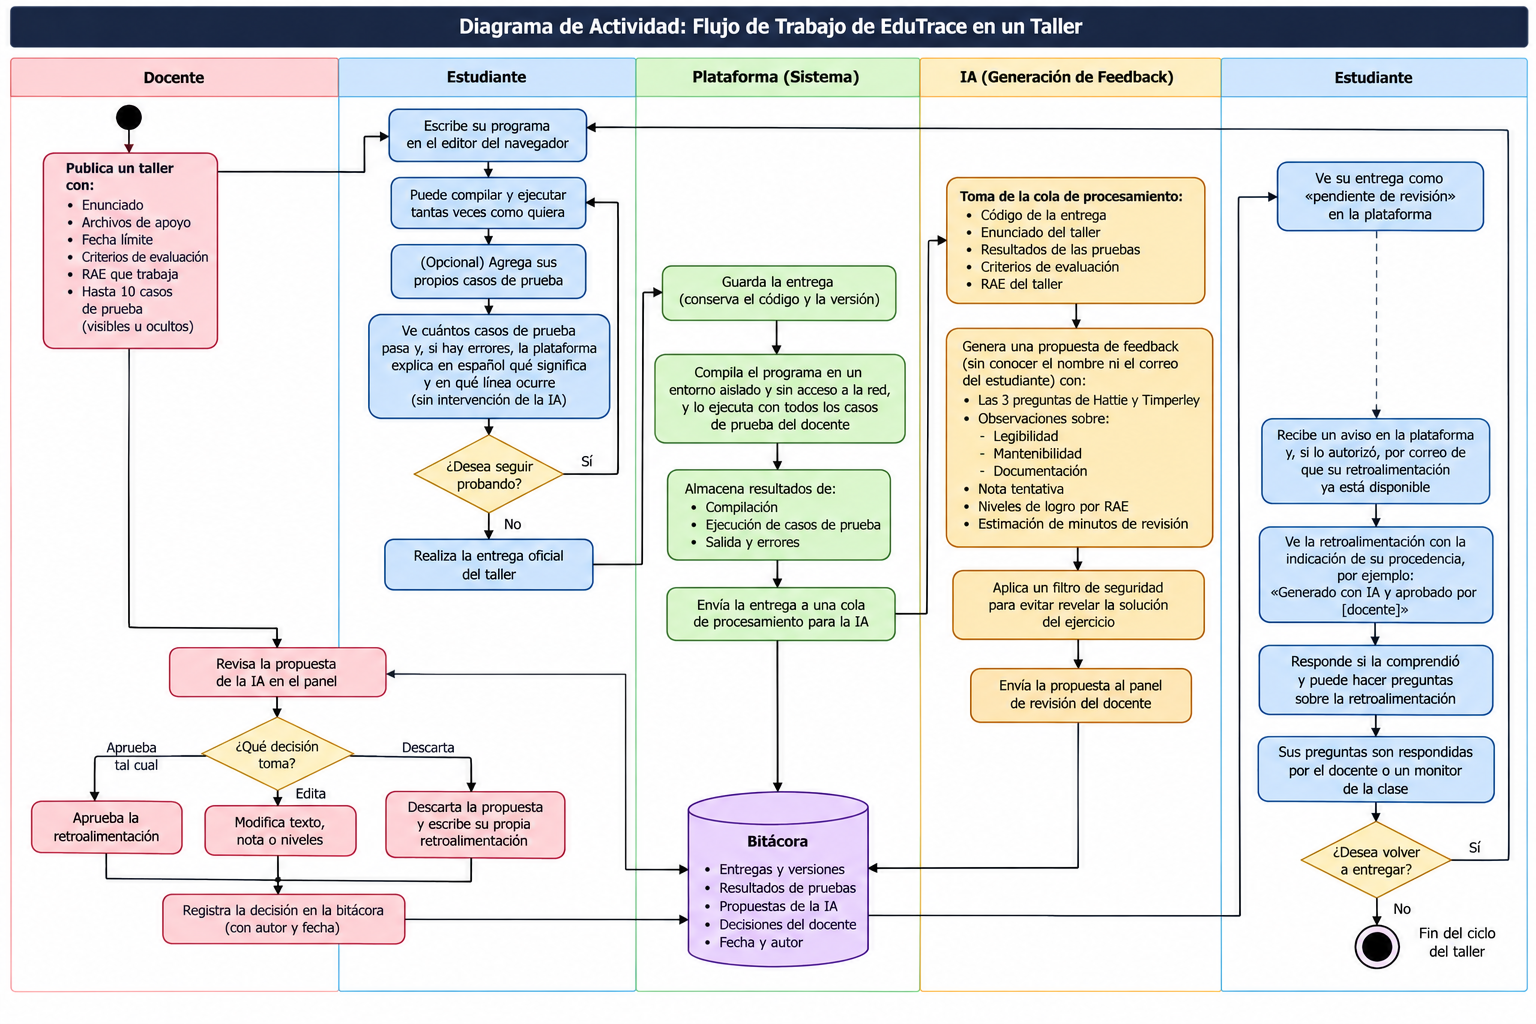
\includegraphics[width=\textwidth]{images/Actividad_Componentes.png}
	\caption{Diagrama de actividad del flujo de trabajo de EduTrace en un taller}
	\label{fig:actividad_componentes}
\end{figure*}

La plataforma tiene dos formas de usar la IA que el profesor puede configurar para cada clase.
En el modo supervisado que es el modo por defecto el estudiante no puede consultar directamente a la IA y solo recibe la retroalimentación que apruebe el docente, de esta forma se concreta el principio de que la IA propone y el profesor decide.
En el modo inmediato, el estudiante puede obtener retroalimentación, pistas progresivas que nunca dan la solución y conversar con un tutor de IA, con un límite de solicitudes por hora.
Este modo es una excepción que el docente activa de forma explícita tras una advertencia, y queda registrada en la bitácora; también puede marcar un taller como evaluación para que la IA no esté disponible hasta su fecha límite.

Frente al mockup del PMV 0.0 Beta definido en la fase de análisis, el prototipo conserva la idea central, una vista del estudiante con retroalimentación de tipo feed-forward y una vista del docente en la que este revisa y aprueba antes de que el estudiante reciba el resultado.
Sin embargo, el desarrollo amplió y concretó esa propuesta en varios aspectos, ampliando las funcionalidades y la interfaz de diferentes formas.
Se incorporaron el editor y la compilación en el navegador con casos de prueba, que el mockup no contemplaba al momento de realizarlo, se definieron los dos modos de IA descritos anteriormente, se añadió el rol del monitor, que comenta el código y responde preguntas sin calificar, y se agregaron indicadores para el docente, como el tiempo real de revisión, la comprensión de la retroalimentación y los errores frecuentes del curso comparando los diferentes elementos.
La Figura 10 se muestra una vista del prototipo que diferencia la vista de revisión del docente con respecto a la del mockup beta.

\begin{figure}[ht]
	\centering
	\placeholderfig{images/MuestraEdu.png}{Vista del docente en el prototipo de EduTrace}
	\caption{Vista del docente en el prototipo de EduTrace}
	\label{fig:muestra_prototipo}
\end{figure}

\subsection{Usuarios de la Plataforma}
Edutrace fue concebida para ser utilizada por tres tipos de usuarios: estudiantes, docentes y monitores. Añadiendo un cuarto rol interesado que es la propia universidad y sus integrantes como parte de la comunidad academica interesada, del mismo modo fue diseñada para el curso de Introduccion a la programacion de la Pontificia Universidad Javeriana, pero puede ser escalada hacia otros cursos y universidades con sus respectivos cursos introductorios de programacion, 
al ser orientado hacia los estudiantes de la PUJ se tomaron decisiones de diseño y desarrollo que se ajustan a la experiencia de usuario de los estudiantes y docentes de la institucion, como por ejemplo la inclusion de C++ como lenguaje de desarrollo y con los RAE esperados para el curso de introduccion a la programacion, y la inclusion de los casos de prueba y el syllabus del curso en la plataforma, que permiten que la IA pueda generar retroalimentacion de calidad y ajustada a los criterios del curso.
Como se mostró en el contexto, una parte importante de los estudiantes percibe el curso como difícil y el 69,6 \% recurre a la IA como su principal fuente de ayuda, mientras que el docente debe dar retroalimentación de calidad a muchos estudiantes en poco tiempo.
Por eso, la plataforma reconoce a los tres tipos de usuarios con necesidades y permisos distintos el estudiante, que es el beneficiario de la retroalimentación, el profesor, que es quien decide y retroalimenta, y el monitor, que apoya el acompañamiento sin tomar un rol en la calificación pero si en la retroalimentación de forma directa.
La Tabla~\ref{tab:usuarios} hace un analisis qué necesita cada uno y qué puede hacer dentro de la plataforma.

\begin{table*}[t]
\centering
\small
\caption{Usuarios de EduTrace, necesidades y funciones.}
\label{tab:usuarios}
\begin{tabular}{|p{2cm}|p{5.2cm}|p{9.5cm}|}
\hline
\textbf{Usuario} & \textbf{Qué necesita} & \textbf{Qué puede hacer} \\
\hline
Estudiante &
Saber qué está mal en su código y cuál es el siguiente paso para mejorarlo, sin recibir la solución de forma directa, con retroalimentación oportuna y en un lenguaje comprensible para cualquier nivel. &
Escribir, compilar y ejecutar código en el navegador, ver los resultados de los casos de prueba y los errores explicados en español, entregar talleres practicos, practicar con un banco de ejercicios preestablecido, consultar su historial, sus notas y su nivel por RAE, indicar si entendió la retroalimentación y hacer preguntas, en el modo inmediato, pedir retroalimentación, pistas y conversar con un tutor de IA. \\
\hline
Profesor &
Dar retroalimentación de calidad a muchos estudiantes sin perder el control sobre la nota ni sobre su criterio pedagógico. &
Crear materias, clases, talleres, casos de prueba, criterios y RAE, revisar, editar, aprobar o descartar las propuestas de la IA, definir el modo de IA de cada clase, consultar indicadores, errores frecuentes, alertas tempranas y código similar entre entregas, responder preguntas, exportar notas, compartir la materia con otros profesores y copiarla para el siguiente periodo. \\
\hline
Monitor &
Apoyar al profesor en el acompañamiento de los estudiantes sin asumir un rol directo en la calificación. &
Ver las entregas de las clases que tiene asignadas, comentar y marcar el código, y responder las preguntas de los estudiantes.  \\
\hline
\end{tabular}
\end{table*}
Además de estos tres usuarios, la institución es un actor interesado que no usa la plataforma directamente, pero del que depende su adopción tanto en modelo de negocio y de forma practica cumpliendo las restricciones y algunos requisitos no funcionales.
En la tabla de actores de la fase de análisis se identificó un cierto equilibrio y separacion de responsabilidades entre quien se beneficia de la retroalimentación (el estudiante), quien decide sobre ella (el profesor) y quien sostiene la solución (la universidad).
En EduTrace, la institución es la encargada de alojar el servidor, de responder por el tratamiento de los datos personales de los estudiantes según la Ley 1581 de 2012 y de autorizar la integración con su plataforma académica, Campus Virtual.
Por esta razón, aunque no aparece como un rol dentro de la plataforma, su papel es determinante  en el modelo de negocio que Edutrace quiere realizar.

\subsection{Arquitectura de la Plataforma}
La arquitectura de EduTrace sigue un modelo cliente-servidor organizado como un monolito modular, en el que todos los componentes se ejecutan en un único servidor.
El navegador del estudiante o del profesor se comunica con Caddy, que actúa como proxy inverso con HTTPS y reparte las peticiones: las páginas las sirve el servidor de Next.js y las peticiones a \texttt{/api} las atiende el backend en Go.
El backend se divide en módulos con responsabilidades separadas: \texttt{handler} expone la API REST y el envío por partes de la retroalimentación (SSE), \texttt{compiler} compila y prueba el código en un entorno aislado, \texttt{auth} concentra los permisos y el acceso a los datos, y \texttt{ai} construye las instrucciones para el modelo y filtra sus respuestas.
Los datos se guardan en SQLite y las propuestas de la IA las genera un modelo local a través de Ollama, de modo que ningún dato sale del servidor.
La Figura~\ref{fig:arquitectura} muestra estos componentes y cómo se relacionan.

\begin{figure*}[t]
\centering
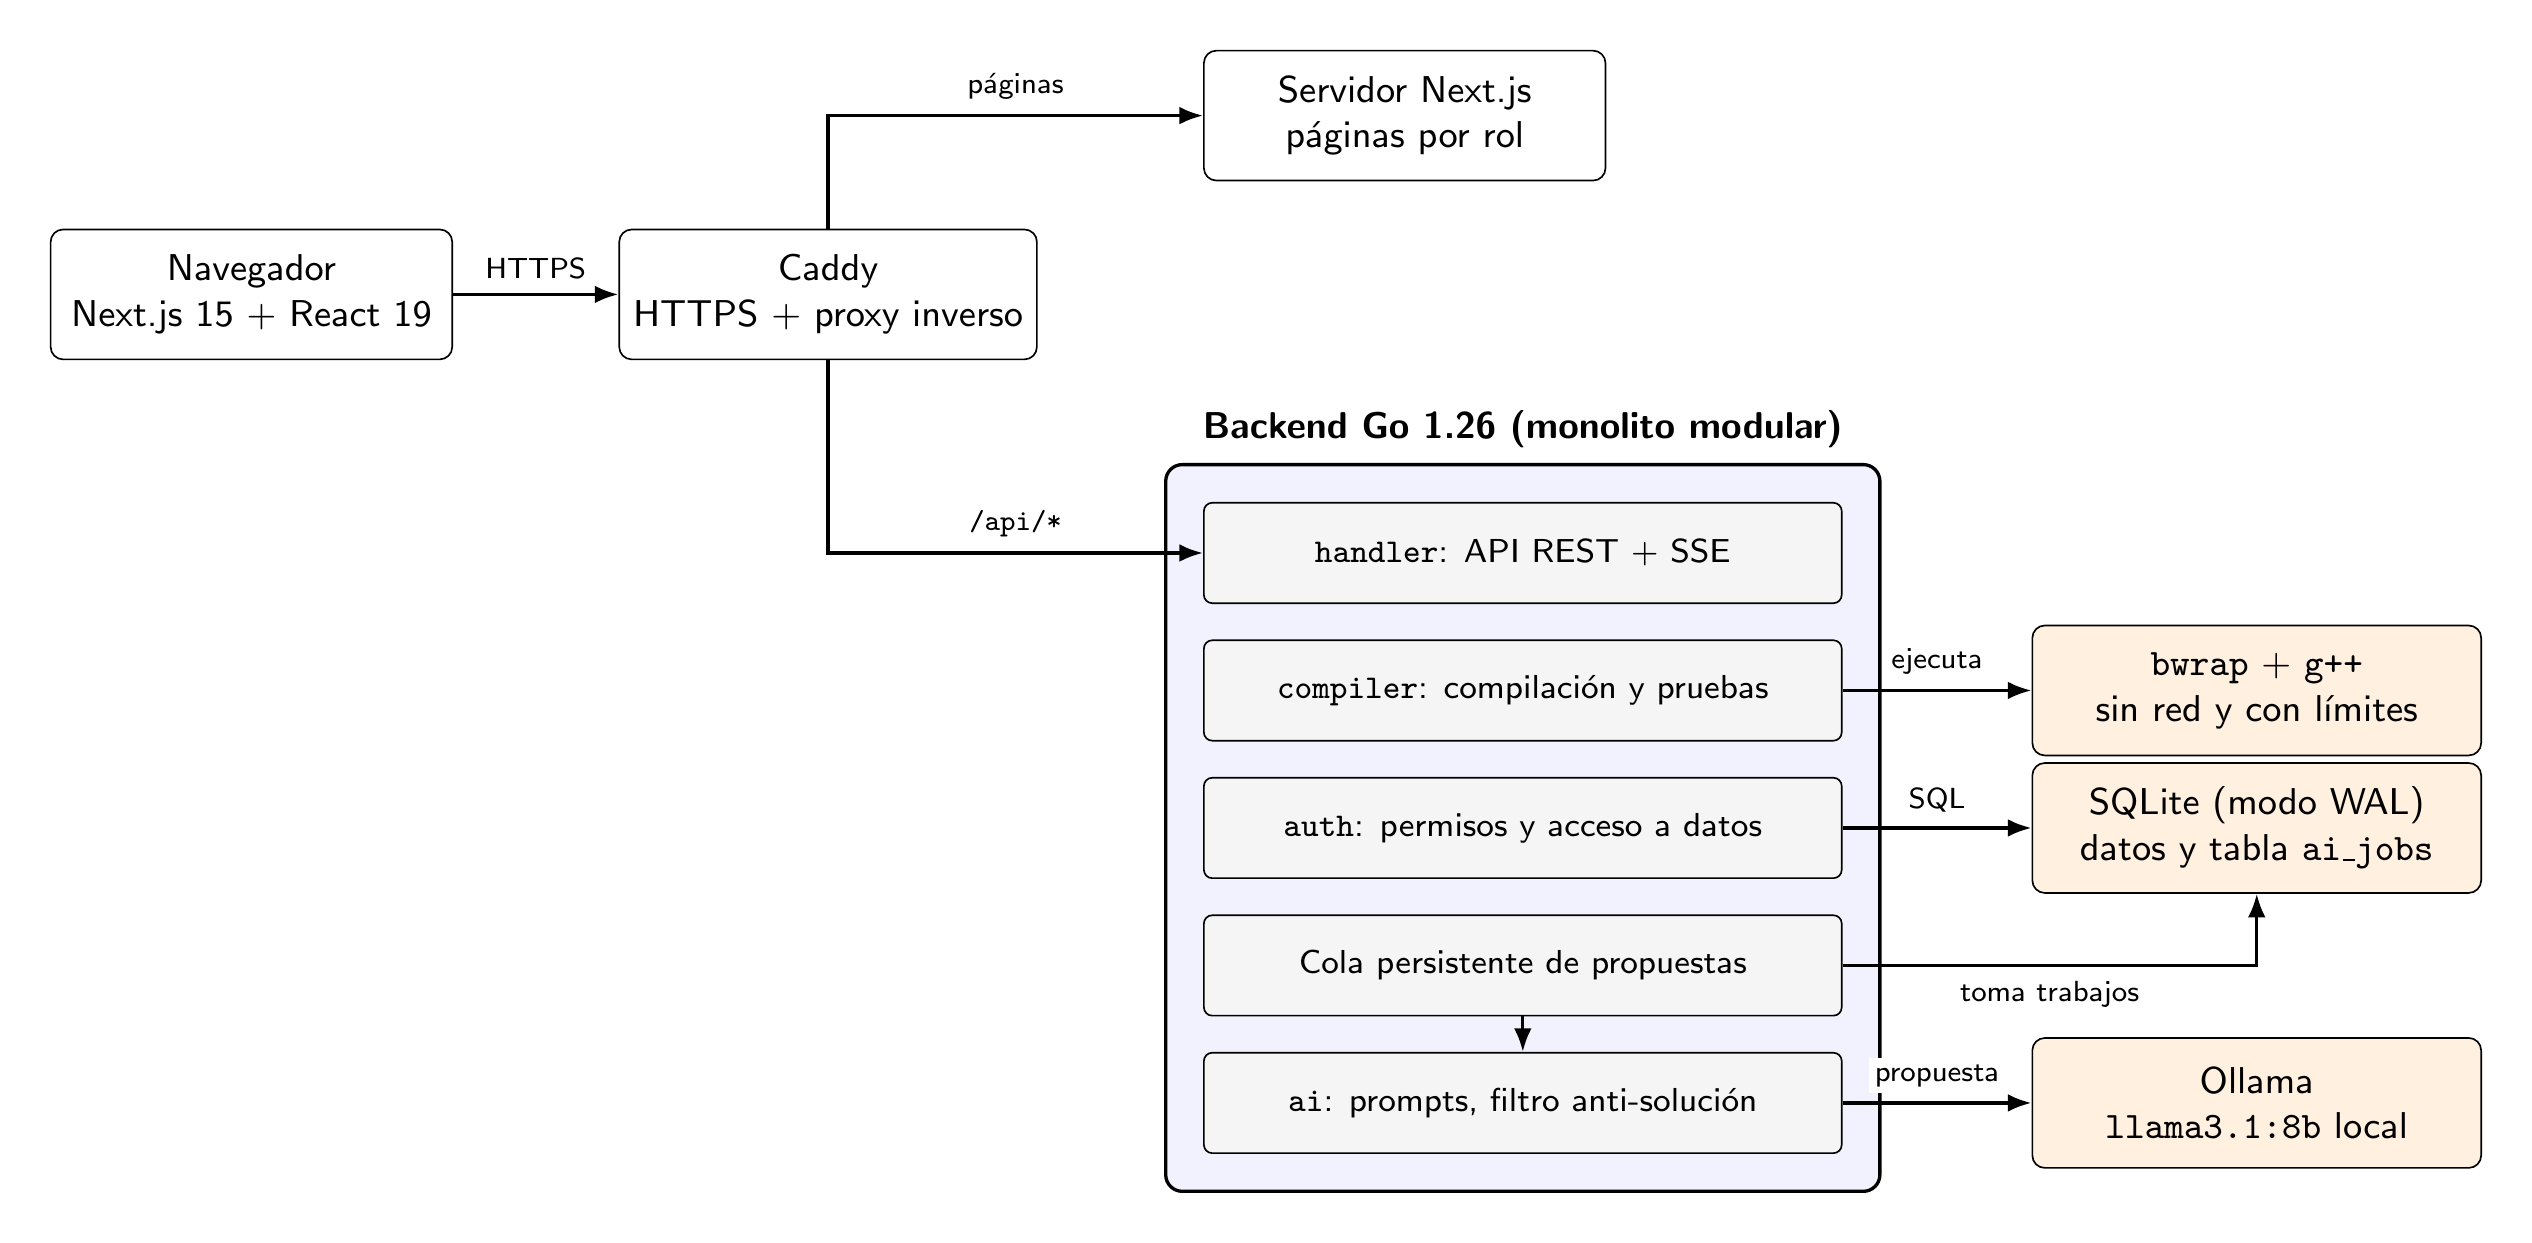
\includegraphics[width=\textwidth]{images/arquitectura_edutrace.png}
\caption{Arquitectura de EduTrace con los diferentes componentes.}
\label{fig:arquitectura}
\end{figure*}
Las decisiones de arquitectura se tomaron a partir de los requisitos definidos en la fase de análisis.
La Tabla~\ref{tab:decisiones} resume las principales decisiones tomadas.
\begin{table*}[t]
\centering
\small
\caption{Principales decisiones de arquitectura y su justificación}
\label{tab:decisiones}
\begin{tabular}{|p{3.6cm}|p{13.6cm}|}
\hline
\textbf{Decisión} & \textbf{Justificación} \\
\hline
Monolito modular en Go &
El equipo es pequeño y todo corre en un solo servidor, así que dividir la plataforma en varios servicios solo habría complicado las cosas. Go deja todo en un único programa, fácil de instalar, y aguanta bien varias compilaciones al mismo tiempo. \\
\hline
SQLite WAL &
No hace falta instalar ni mantener un servidor de base de datos, toda la información queda en un archivo que se respalda y se verifica cada día. El modo WAL permite que varias personas consulten al tiempo sin estorbarse. \\
\hline
IA local con Ollama (\texttt{llama3.1:8b}) &
El código de los estudiantes no sale del servidor y el modelo nunca conoce su nombre ni su correo, algo que importa cuando se trabaja con datos de personas como en este caso. \\
\hline
Ejecución aislada con \texttt{bwrap} &
Cualquier programa que envía un estudiante podría tener un error o hacer algo indebido, así que se ejecuta sin acceso a la red y con límites de procesos, memoria, tiempo y tamaño de archivos. Si el aislamiento no funciona, el servidor no arranca, es preferible no ofrecer el servicio antes que correr código sin protección. \\
\hline
Cola persistente de propuestas &
La entrega y su turno en la cola se guardan al mismo tiempo, así que ningún trabajo se pierde aunque la IA falle o el servidor se reinicie. Si algo sale mal, la plataforma lo intenta hasta tres veces y si aun así no lo logra, le avisa al docente para que sepa qué pasó. \\
\hline
Caddy con HTTPS &
Deja toda la plataforma en una sola dirección web segura y renueva los certificados por su cuenta. \\
\hline
Next.js 15 y React 19 &
Stack tecnológico que facilita armar pantallas distintas para cada rol (estudiante, profesor y monitor) y mantener páginas livianas, lo que ayuda a quienes tienen una conexión lenta. La accesibilidad según WCAG 2.1 AA se revisa de forma automática cada vez que se integra un cambio. \\
\hline
\end{tabular}
\end{table*}

En cuanto al diseño interno, se aplicaron varios patrones de arquitectura y de diseño.
A nivel de arquitectura, además del estilo cliente-servidor y el proxy inverso, el backend se organiza por capas: la presentación en Next.js, la API en \texttt{handler}, los servicios de compilación e IA en \texttt{compiler} y \texttt{ai}, y el acceso a datos en \texttt{auth}.
A nivel de diseño, se usaron los siguientes patrones:
\begin{itemize}
  \item \textbf{Middleware (cadena de decoradores):} los permisos se aplican envolviendo cada ruta con funciones que verifican la sesión y el rol (\texttt{RequireAuth}, \texttt{RequireRole}, \texttt{RequireLearner}); lo mismo ocurre con la compresión y las cabeceras de seguridad.
  \item \textbf{Repositorio:} el acceso a la base de datos se concentra en un único componente (\texttt{Store}), y cada consulta filtra por dueño, clase o monitor asignado, de modo que los permisos se aplican en el propio SQL.
  \item \textbf{Productor-consumidor con cola persistente:} cada entrega produce un trabajo en la tabla \texttt{ai\_jobs} y un trabajador en segundo plano lo consume, con reintentos y recuperación tras un reinicio.
  \item \textbf{Máquina de estados:} cada revisión pasa de borrador a devuelta solo por una acción del docente, y cada trabajo de la cola pasa por los estados pendiente, procesando, lista, error u omitida. Así, el principio de que el profesor decide queda garantizado por el sistema, no solo por la interfaz.
  \item \textbf{Tubería de filtros:} la respuesta del modelo pasa por filtros sucesivos que completan las tres preguntas de Hattie y Timperley si faltan, agregan las observaciones de calidad y eliminan la solución del ejercicio.
  \item \textbf{Semáforo:} un número máximo de programas puede compilarse o ejecutarse al mismo tiempo, para que una carga alta no tumbe el servidor.
  \item \textbf{Inyección de dependencias:} los módulos reciben sus dependencias al construirse, lo que permite probarlos de forma aislada.
  \item \textbf{Proveedor de contexto en React:} la sesión del usuario se comparte entre las páginas mediante un contexto de autenticación.
\end{itemize}

Frente al diagrama de actividad de la Figura~\ref{fig:diagrama_actividad} de la fase anterior, la arquitectura implementada introduce dos cambios.
En ese diagrama, un orquestador coordinaba la compilación y la IA y entregaba las sugerencias directamente al estudiante.
En el prototipo, ese orquestador desaparece como componente independiente y su función se divide en dos partes, la compilación y los casos de prueba se ejecutan de inmediato en el backend cuando el estudiante entrega, y la propuesta de la IA se genera después, de forma asíncrona, a través de la cola persistente.
El segundo cambio que se introduce es que la salida de la IA ya no llega al estudiante, sino que queda como borrador hasta que el docente la aprueba, la edita o la descarta.
De esta manera, la arquitectura incorpora de forma explícita el principio de \textit{human-in-the-loop} que guío todo el proyecto.

\subsection{Cumplimiento de Requisitos}
Siguiendo la ciencia del diseño, el prototipo se evalúa frente a los requisitos definidos en la fase de análisis, que funcionan como los objetivos de la solución.
Esta evaluación técnica revisa, para cada requisito, si existe una implementación y una prueba o medición que lo demuestre, y distingue lo que ya se cumple en el código de lo que depende de una auditoría y lo que se puede desarrollar a futuro, del uso con estudiantes reales o de la institución.
Para ello se usaron cinco estados: \textit{cumple}, cuando hay implementación y una prueba que lo verifica, \textit{instrumentado}, cuando la plataforma ya mide el criterio pero falta usarla con estudiantes, \textit{parcial}, cuando se cubre solo una parte, \textit{pendiente}, cuando aún no está implementado, y \textit{fuera del código}, cuando depende de un análisis o de una decisión institucional.

Como resultado, el prototipo cumple los 23 requisitos funcionales y 12 de los 16 requisitos no funcionales.
De los cuatro restantes, el RNF-01 está implementado pero requiere una auditoría legal, el RNF-02 se cumple de forma parcial porque falta la evaluación de impacto de la IA, el RNF-09 está instrumentado a la espera de su uso con estudiantes, y el RNF-13, la integración con Campus Virtual, queda pendiente.
Las Tablas~\ref{tab:cumplimiento} y~\ref{tab:cumplimiento_rnf} resumen el estado de cada requisito de acuerdo a la fase de análisis establecida.


\begin{table*}[t]
\centering
\footnotesize
\caption{Cumplimiento de los requisitos funcionales}
\label{tab:cumplimiento}
\begin{tabular}{|p{1.2cm}|p{4.6cm}|p{2.2cm}|p{8.2cm}|}
\hline
\textbf{ID} & \textbf{Requisito} & \textbf{Estado} & \textbf{Cómo se cumple} \\
\hline
RF-01 & Retroalimentación para cada entrega & Cumple & Cada entrega oficial entra a la cola y recibe una propuesta de la IA. \\ \hline
RF-02 & Tres preguntas de Hattie y Timperley & Cumple & Toda propuesta se organiza en ¿hacia dónde voy?, ¿cómo voy? y ¿qué sigue?, si falta una sección, se completa. \\ \hline
RF-03 & «¿Qué sigue?» en todas las salidas & Cumple & Si el modelo la omite, se agrega una pista según el resultado de la entrega. \\ \hline
RF-04 & Corrección con casos de prueba & Cumple & Hasta diez casos por taller, visibles u ocultos, ejecutados al compilar y al entregar. \\ \hline
RF-05 & Observación sobre legibilidad & Cumple & Un analizador revisa sangría, nombres y líneas largas, y pasa los hallazgos a la IA. \\ \hline
RF-06 & Observación sobre mantenibilidad & Cumple & El analizador detecta código repetido, variables globales y funciones muy largas. \\ \hline
RF-07 & Observación sobre documentación & Cumple & El analizador revisa la presencia de comentarios. \\ \hline
RF-08 & Pistas orientadas al razonamiento & Cumple & Las instrucciones del modelo exigen preguntas guía y pistas graduadas. \\ \hline
RF-09 & No revelar la solución & Cumple & Un filtro elimina la solución de la propuesta y de las respuestas en vivo. \\ \hline
RF-10 & Estado «pendiente de revisión» & Cumple & Toda revisión empieza como borrador y el estudiante no la ve hasta que se aprueba. \\ \hline
RF-11 & Editar antes de entregar & Cumple & Texto, nota y niveles por RAE son editables en el panel de revisión. \\ \hline
RF-12 & Aprobación registrada & Cumple & La aprobación queda en la bitácora con autor, fecha, nota y origen del texto. \\ \hline
RF-13 & Descarte registrado & Cumple & El descarte elimina la propuesta, impide regenerarla y queda en la bitácora. \\ \hline
RF-14 & Configurar criterios & Cumple & Criterios por taller, RAE por materia y casos de prueba definidos por el profesor. \\ \hline
RF-15 & La rúbrica se refleja en la salida & Cumple & La propuesta usa los criterios, los RAE y los casos de prueba del taller. \\ \hline
RF-16 & Ejecución automática & Cumple & Cada entrega dispara compilación, pruebas y propuesta sin intervención manual. \\ \hline
RF-17 & Separar lo formativo de lo sumativo & Cumple & La IA no pone notas en el texto; la nota es un campo aparte que define el profesor. \\ \hline
RF-18 & Aviso de participación de la IA & Cumple & Toda salida de la IA lleva su aviso, y cada revisión indica si hubo IA. \\ \hline
RF-19 & Contenido de IA marcado & Cumple & El origen del texto queda como IA, IA editada o docente, y el estudiante lo ve. \\ \hline
RF-20 & Bitácora de intervenciones & Cumple & Se registran autor, acción y fecha de cada propuesta, aprobación, descarte y cambio. \\ \hline
RF-21 & Errores frecuentes del curso & Cumple & Errores de compilación, ejecución y casos de prueba agrupados por clase o materia. \\ \hline
RF-22 & Aclaración sobre la retroalimentación & Cumple & El estudiante pregunta debajo de la retroalimentación y responde el profesor o un monitor. \\ \hline
RF-23 & Iterar & Cumple & El estudiante puede volver a entregar, y cada versión tiene su revisión. \\ \hline
\end{tabular}
\end{table*}

\begin{table*}[t]
\centering
\footnotesize
\caption{Cumplimiento de los requisitos no funcionales y las restricciones de viabilidad}
\label{tab:cumplimiento_rnf}
\begin{tabular}{|p{1.2cm}|p{4.6cm}|p{2.2cm}|p{8.2cm}|}
\hline
\textbf{ID} & \textbf{Requisito} & \textbf{Estado} & \textbf{Cómo se cumple} \\
\hline
RNF-01 & Ley 1581 de 2012 & Implementado, falta auditoría & Autorización versionada, política pública, descarga y eliminación de datos y borrado automático al cerrar el periodo. \\ \hline
RNF-02 & Circular 002 de 2024 (SIC) & Parcial & Supervisión humana, transparencia y modelo local, falta la evaluación de impacto de la IA en plataforma. \\ \hline
RNF-03 & Confidencialidad del código & Cumple en el código & Ejecución aislada sin red y con límites, permisos filtrados en SQL y cabeceras de seguridad. \\ \hline
RNF-04 & Confidencialidad de datos personales & Cumple en el código & Contraseñas guardadas con hash, sesión segura y respaldos diarios verificados, que pueden cifrarse. \\ \hline
RNF-05 & Control de lo que recibe la IA & Cumple & El modelo es local y nunca recibe el nombre ni el correo del estudiante. \\ \hline
RNF-06 & Validación docente de la retroalimentación & Cumple en modo supervisado & En el modo predeterminado, el estudiante solo recibe lo que el profesor aprueba. \\ \hline
RNF-07 & Docente como decisor final & Cumple & Aprobar, editar, descartar y calificar son acciones exclusivas del profesor. \\ \hline
RNF-08 & Tiempo de revisión por entrega & Cumple & La IA estima los minutos de revisión y la plataforma mide el tiempo real. \\ \hline
RNF-09 & Lenguaje comprensible para CS1 & Instrumentado & Cada retroalimentación pregunta si se entendió; meta de al menos 80 \% de respuestas afirmativas. \\ \hline
RNF-10 & Procesar el volumen del curso & Cumple & Prueba de carga con 200 entregas, peor demora de 1 h 21 min frente a un umbral de 5 h. \\ \hline
RNF-11 & Retroalimentación a tiempo & Cumple & Se mide el tiempo entre la entrega y la aprobación, con un umbral de 5 h. \\ \hline
RNF-12 & Conectividad limitada & Cumple & Páginas de 206 a 237 KB y respuestas comprimidas de menos de 2 KB. \\ \hline
RNF-13 & Integración con la plataforma institucional & Pendiente & Requiere el registro de EduTrace en Campus Virtual (Brightspace), por ahora exporta en CSV ciertos elementos. \\ \hline
RNF-14 & Conservar la entrega si falla la IA & Cumple & La entrega se guarda antes de la IA y la cola reintenta sin modificarla. \\ \hline
RNF-15 & Avisar al docente si falla la IA & Cumple & Aviso en el tablero, botón para reintentar y alertas del servidor cada 5 minutos. \\ \hline
RNF-16 & Vínculo docente-estudiante & Cumple & La revisión muestra quién la aprobó y el estudiante puede preguntarle directamente. \\ \hline
\end{tabular}
\end{table*}

La evaluación se apoya en tres fuentes de evidencia.
La primera es una prueba de carga con 200 entregas simultáneas, ejecutada con el modelo \texttt{llama3.1:8b} en una GPU RTX 3050 de 6 GB: las 200 entregas se compilaron con sus casos de prueba en 78 segundos y todas las propuestas quedaron listas sin errores, con una mediana de 23,5 segundos por propuesta y una peor demora de 1 h 21 min, frente a un umbral de 5 horas.
La segunda son 63 pruebas automatizadas del backend, que verifican, entre otros aspectos, el aislamiento del código, los límites del entorno de ejecución, el filtro que impide revelar la solución, los permisos por rol y la restauración de los respaldos.
La tercera es una revisión de accesibilidad según el estándar WCAG 2.1 AA sobre las páginas públicas, las del estudiante y las del profesor.
Las pruebas automatizadas y la revisión de accesibilidad se ejecutan en cada cambio mediante integración continua, junto con un análisis de vulnerabilidades de las dependencias, de modo que una versión que falle alguna de ellas no se despliega.

\subsection{Validación con Usuarios}


\section{Fase 4: Proyección}


\subsection{Recursos necesarios}


\subsection{Roadmap tecnológico}


\subsection{Investigación, desarrollo e innovación (I+D+i)}


\subsection{Plan de negocio}
\subsubsection{Plan de mercadeo}

\subsubsection{Plan financiero}

\subsubsection{Estrategias de financiación}


\subsection{Riesgos}


\subsection{Conclusiones y trabajo futuro}


%\addtolength{\textheight}{-12cm}   % This command serves to balance the column lengths
                                  % on the last page of the document manually. It shortens
                                  % the textheight of the last page by a suitable amount.
                                  % This command does not take effect until the next page
                                  % so it should come on the page before the last. Make
                                  % sure that you do not shorten the textheight too much.

%%%%%%%%%%%%%%%%%%%%%%%%%%%%%%%%%%%%%%%%%%%%%%%%%%%%%%%%%%%%%%%%%%%%%%%%%%%%%%%%



%%%%%%%%%%%%%%%%%%%%%%%%%%%%%%%%%%%%%%%%%%%%%%%%%%%%%%%%%%%%%%%%%%%%%%%%%%%%%%%%



%%%%%%%%%%%%%%%%%%%%%%%%%%%%%%%%%%%%%%%%%%%%%%%%%%%%%%%%%%%%%%%%%%%%%%%%%%%%%%%%


\begin{thebibliography}{99}

\bibitem{1} J. Hattie and H. Timperley, "The power of feedback," \textit{Rev. Educ. Res.}, vol. 77, no. 1, pp. 81–112, Mar. 2007.

\bibitem{2} Superintendencia de Industria y Comercio, “Circular Externa No. 002 del 21 de agosto de 2024: Lineamientos sobre el tratamiento de datos personales en sistemas de inteligencia artificial,” Bogotá, Colombia, 2024.

\bibitem{3} Congreso de la República de Colombia, “Ley Estatutaria 1581 de 2012, por la cual se dictan disposiciones generales para la protección de datos personales,” \textit{Diario Oficial No. 48.587}, Bogotá, Colombia, 17 de oct. de 2012.

\bibitem{4} F. Miao and W. Holmes, \textit{Guidance for generative AI in education and research}. Paris, France: UNESCO, 2023. [Online].

\bibitem{5} D. R. Sadler, "Formative assessment and the design of instructional systems," \textit{Instructional Sci.}, vol. 18, no. 2, pp. 119–144, 1989.

\bibitem{6} P. Black and D. Wiliam, "Inside the black box: Raising standards through classroom assessment," \textit{Phi Delta Kappan}, vol. 92, no. 1, pp. 81–90, 2010.

\bibitem{7} D. J. Nicol and D. Macfarlane-Dick, "Formative assessment and self-regulated learning: A model and seven principles of good feedback practice," \textit{Stud. High. Educ.}, vol. 31, no. 2, pp. 199–218, 2006.

\bibitem{8} S. Shubha, H. R. Gopala Krishna Murthy, and S. Shubhakar, "AI-based automated grading and feedback systems: Technologies, challenges and future directions in higher education," \textit{Int. J. Res. Innov. Appl. Sci.}, vol. 11, no. 2, pp. 267–279, Feb. 2026.

\bibitem{9} K. Ala-Mutka, "A survey of automated assessment approaches for programming assignments," \textit{Comput. Sci. Educ.}, vol. 15, no. 2, pp. 83–102, 2005.

\bibitem{10} H. Keuning, J. Jeuring, and B. Heeren, "A systematic literature review of automated feedback generation for programming exercises," \textit{ACM Trans. Comput. Educ.}, vol. 19, no. 1, art. 3, 2018.

\bibitem{11} M. Messer, N. C. C. Brown, M. Kölling, and M. Shi, "Automated grading and feedback tools for programming education: A systematic review," \textit{ACM Trans. Comput. Educ.}, 2024, doi: 10.1145/3636515.

\bibitem{12} S. S. Lee and R. L. Moore, "Harnessing generative AI (GenAI) for automated feedback in higher education: A systematic review," \textit{Online Learn.}, vol. 28, no. 3, pp. 82–104, Sep. 2024.

\bibitem{13} Z. Ma, C. Du, Q. Lao, and X. Xie, "Generative artificial intelligence: Applications and future prospects in dentistry," \textit{Int. Dent. J.}, vol. 76, no. 1, art. 108276, 2026.

\bibitem{14} Organización de las Naciones Unidas para la Educación, la Ciencia y la Cultura, \textit{Recomendación sobre la ética de la inteligencia artificial}. Paris, Francia: UNESCO, 2021.

\bibitem{15} E. F. Risko and S. J. Gilbert, "Cognitive offloading," \textit{Trends Cogn. Sci.}, vol. 20, no. 9, pp. 676–688, Sep. 2016.

\bibitem{16} Ministerio de Educación Nacional, "Equidad e inclusión: retos de la inteligencia artificial en los sistemas educativos del mundo," Comunicado de prensa, 5 de dic. de 2024.

\bibitem{17} GADE: Revista Científica, "Inteligencia artificial y brecha digital en la educación superior: revisión internacional con foco en Colombia," \textit{GADE: Rev. Cient.}, vol. 6, no. 1, pp. 95–116, 2026.

\bibitem{18} "Artificial intelligence and cost reduction in public higher education: A scoping review of emerging evidence," preprint, arXiv:2604.04741, 2026.

%--- Referencias añadidas de la presentación ---%
\bibitem{19} D. Calderón Gómez, “Jóvenes y desigualdad digital: Las brechas de acceso, competencias y uso,” Centro Reina Sofía de Fad Juventud, 2020. [En línea]. Disponible: https://www.centroreinasofia.org/blog/analisis-y-debate/jovenes-y-desigualdad-digital-las-brechas-de-access-competencias-y-uso/

\bibitem{20} Congreso de la República de Colombia, “Ley 23 de 1982, sobre derechos de autor,” \textit{Diario Oficial}, Bogotá, Colombia, 28 de enero de 1982.

\bibitem{21} M. Jukiewicz, “A systematic comparison of large language models for automated assignment assessment in programming education,” preprint, arXiv:2509.26483, 2025.

\bibitem{22} A. Milne, “ChatGPT in the classroom: Exploring its potential and limitations in a Functional Programming course,” preprint, arXiv:2401.11166, 2024.

\bibitem{23} K. Mohamed, M. Yousef, W. Medhat, E. H. Mohamed, G. Khoriba, y T. Arafa, “Hands-on analysis of using large language models for the auto evaluation of programming assignments,” \textit{Information Systems}, vol. 128, Art. 102473, 2025.

\bibitem{24} C. Watson y F. W. B. Li, “Failure rates in introductory programming revisited,” en \textit{Proc. 2014 Conf. Innovation Technol. Comput. Sci. Educ. (ITiCSE '14)}, Uppsala, Sweden, 2014, pp. 39–44.




%SE PUEDE AÑADIR COMO UN PARRAFO SOBRE LO LUCRATIVO DE LA IDEA EN EL AMBITO ECONOMICO
%\bibitem{31} Precedence Research, “Artificial intelligence in education market size, share, and trends 2024 to 2034,” 2024. [En línea]. Disponible: https://www.precedenceresearch.com

%SE PUEDE AÑADIR COMO UN PARRAFO SOBRE LO LUCRATIVO DE LA IDEA EN EL AMBITO ECONOMICO
%\bibitem{33} Mordor Intelligence, “Artificial Intelligence in Education Market Size \& Share Analysis - Industry Research Report - Growth Trends \& Forecasts (2024 - 2029),” 2024. [En línea]. Disponible: https://www.mordorintelligence.com/industry-reports/ai-in-education-market

%\bibitem{27} F. J. Jiménez-Mejía, A. G. Pesantes-Pincay, A. S. Menéndez-Menéndez, y J. A. Macías-Vinces, “La brecha digital en la educación virtual: Un análisis de sus causas y consecuencias,” Revista Científica Multidisciplinaria Arbitrada Yachasun, vol. 8, no. 15 Ed. Esp., pp. 69–86, 2024. doi: 10.46296/yc.v8i15edespdic.0554.

%\bibitem{8} GADE: Revista Científica, ISSN-e 2745-2891, Vol. 6, Nº. 1, 2026 (Ejemplar dedicado a: Education Without Borders), págs. 95-116

%\bibitem{9}  Malouff, J. M., \& Thorsteinsson, E. B. (2016). Bias in grading: A meta-analysis of experimental research findings. Australian Journal of Education, 60(3), 245-256.

%\bibitem{10} Butler, R. (1987). Task-involving and ego-involving properties of evaluation: Effects of different feedback conditions on motivational perceptions, interest, and performance. Journal of Educational Psychology, 79(4), 474–48

%\bibitem{2} Carless, D., \& Boud, D. (2018). The development of student feedback literacy: enabling uptake of feedback. Assessment \& Evaluation in Higher Education, 43(8), 1315–1325

%REVISAR
%\bibitem{26} EDUCAUSE, “2025 EDUCAUSE AI landscape study,” 2025. [En línea]. Disponible: https://www.educause.edu

\end{thebibliography}




\end{document}
